% ============================================================================
%  ECS414/614 Network Science Theory and Applications - Assignment report
%
%  Every number printed through \val / \vali / \valf / \valp is read from
%  generated/macros.tex, which scripts/09_export_report_assets.py writes from
%  the analysis outputs.  Re-run the pipeline and recompile to refresh them.
% ============================================================================
\documentclass[11pt,a4paper]{article}

\usepackage[T1]{fontenc}
\usepackage[utf8]{inputenc}
\usepackage{mathpazo}
\usepackage[scaled=0.92]{helvet}
\usepackage{microtype}
\usepackage[a4paper,margin=2.3cm]{geometry}
\usepackage{amsmath,amssymb}
\usepackage{graphicx}
\usepackage{booktabs,multirow,array,tabularx}
\usepackage[font=small,labelfont=bf,skip=6pt]{caption}
\usepackage{siunitx}
\usepackage{xfp}
\usepackage{xcolor}
\usepackage{enumitem}
\usepackage{listings}
\usepackage{float}
\usepackage{adjustbox}
\usepackage{fancyhdr}
\usepackage[colorlinks=true,linkcolor=black,citecolor=black,urlcolor=blue!50!black]{hyperref}

\graphicspath{{figures/}}
\setlength{\parskip}{0.4em}
\setlength{\parindent}{0pt}
\setlength{\headheight}{14pt}
\setlist{itemsep=1pt,topsep=3pt,leftmargin=1.6em}
\renewcommand{\arraystretch}{1.08}
\sisetup{group-separator={,},group-minimum-digits=4,group-digits=integer,detect-all}

\pagestyle{fancy}
\fancyhf{}
\fancyhead[L]{\small ECS414/614 Network Science: Assignment}
\fancyhead[R]{\small Structure of the Indian stock market}
\fancyfoot[C]{\small\thepage}
\renewcommand{\headrulewidth}{0.3pt}

\definecolor{codebg}{gray}{0.965}
\lstset{language=Python,basicstyle=\ttfamily\footnotesize,backgroundcolor=\color{codebg},
  frame=single,rulecolor=\color{black!20},columns=fullflexible,keepspaces=true,showstringspaces=false,
  commentstyle=\color{black!55}\itshape,keywordstyle=\bfseries,breaklines=true,aboveskip=6pt,belowskip=4pt,
  xleftmargin=2pt,xrightmargin=2pt}

% ---- numbers produced by the code -----------------------------------------
\makeatletter
% AUTO-GENERATED by scripts/09_export_report_assets.py - do not edit by hand.
\expandafter\def\csname v@A.back_alpha\endcsname{1.9780630858237513}
\expandafter\def\csname v@A.back_best_full_model\endcsname{power law + cut-off}
\expandafter\def\csname v@A.back_best_tail_model\endcsname{exponential}
\expandafter\def\csname v@A.back_cv\endcsname{2.1339297845247227}
\expandafter\def\csname v@A.back_daic_exp\endcsname{0.0}
\expandafter\def\csname v@A.back_daic_ln\endcsname{6.549718238461082}
\expandafter\def\csname v@A.back_daic_pl\endcsname{30.384391989578603}
\expandafter\def\csname v@A.back_daic_tpl\endcsname{1.9992412707753147}
\expandafter\def\csname v@A.back_edges\endcsname{936}
\expandafter\def\csname v@A.back_er_max_expected\endcsname{11.0}
\expandafter\def\csname v@A.back_er_p_isolated\endcsname{0.013367780713680659}
\expandafter\def\csname v@A.back_er_sd\endcsname{2.061843617677132}
\expandafter\def\csname v@A.back_exp_lambda\endcsname{0.07549153315676835}
\expandafter\def\csname v@A.back_full_alpha\endcsname{1.4766473204097506}
\expandafter\def\csname v@A.back_full_cutoff_scale\endcsname{23.349404220018272}
\expandafter\def\csname v@A.back_full_daic_exp\endcsname{40.15605392123325}
\expandafter\def\csname v@A.back_full_daic_ln\endcsname{16.273002046438705}
\expandafter\def\csname v@A.back_full_daic_pl\endcsname{77.82685262397672}
\expandafter\def\csname v@A.back_full_daic_tpl\endcsname{0.0}
\expandafter\def\csname v@A.back_full_llr_tpl\endcsname{-39.91342631198832}
\expandafter\def\csname v@A.back_full_tpl_alpha\endcsname{0.7579062822974871}
\expandafter\def\csname v@A.back_full_tpl_lambda\endcsname{0.04282764521857327}
\expandafter\def\csname v@A.back_gini\endcsname{0.8207799145299145}
\expandafter\def\csname v@A.back_gof_p\endcsname{0.0}
\expandafter\def\csname v@A.back_isolated\endcsname{250}
\expandafter\def\csname v@A.back_kappa\endcsname{23.800213675213676}
\expandafter\def\csname v@A.back_kmin\endcsname{6}
\expandafter\def\csname v@A.back_ks\endcsname{0.11969124018645855}
\expandafter\def\csname v@A.back_llr_exp\endcsname{-15.19219599478929}
\expandafter\def\csname v@A.back_llr_ln\endcsname{-12.917336875558737}
\expandafter\def\csname v@A.back_llr_tpl\endcsname{-15.192575359401634}
\expandafter\def\csname v@A.back_max\endcsname{50}
\expandafter\def\csname v@A.back_mean\endcsname{4.293577981651376}
\expandafter\def\csname v@A.back_median\endcsname{0.0}
\expandafter\def\csname v@A.back_n\endcsname{436}
\expandafter\def\csname v@A.back_n_connected\endcsname{186}
\expandafter\def\csname v@A.back_ntail\endcsname{89}
\expandafter\def\csname v@A.back_p_exp\endcsname{0.0003417352179307506}
\expandafter\def\csname v@A.back_p_ln\endcsname{0.0012325858141249578}
\expandafter\def\csname v@A.back_p_tpl\endcsname{0.0003172478192734226}
\expandafter\def\csname v@A.back_sd\endcsname{9.162193937225416}
\expandafter\def\csname v@A.back_skew\endcsname{2.769092504878926}
\expandafter\def\csname v@A.back_tail_frac\endcsname{0.20412844036697247}
\expandafter\def\csname v@A.back_top10pct_share\endcsname{0.6629273504273504}
\expandafter\def\csname v@A.back_top1pct_share\endcsname{0.0998931623931624}
\expandafter\def\csname v@A.back_tpl_alpha\endcsname{0.013015888546362276}
\expandafter\def\csname v@A.back_tpl_lambda\endcsname{0.07492865569252613}
\expandafter\def\csname v@A.ladder_n\endcsname{7}
\expandafter\def\csname v@A.ladder_n_pl_plausible\endcsname{2}
\expandafter\def\csname v@A.star_alpha\endcsname{5.101986842124456}
\expandafter\def\csname v@A.star_best_full_model\endcsname{power law + cut-off}
\expandafter\def\csname v@A.star_best_tail_model\endcsname{log-normal}
\expandafter\def\csname v@A.star_cv\endcsname{1.4900696530546687}
\expandafter\def\csname v@A.star_daic_exp\endcsname{1.5467413501866645}
\expandafter\def\csname v@A.star_daic_ln\endcsname{0.0}
\expandafter\def\csname v@A.star_daic_pl\endcsname{6.649341923494717}
\expandafter\def\csname v@A.star_daic_tpl\endcsname{1.0553299834056133}
\expandafter\def\csname v@A.star_edges\endcsname{5096}
\expandafter\def\csname v@A.star_er_max_expected\endcsname{38.0}
\expandafter\def\csname v@A.star_er_p_isolated\endcsname{3.672023192647808e-11}
\expandafter\def\csname v@A.star_er_sd\endcsname{4.703185424454993}
\expandafter\def\csname v@A.star_exp_lambda\endcsname{0.0412335094621841}
\expandafter\def\csname v@A.star_full_alpha\endcsname{1.3179258451028866}
\expandafter\def\csname v@A.star_full_cutoff_scale\endcsname{64.76840825062347}
\expandafter\def\csname v@A.star_full_daic_exp\endcsname{65.75581392730646}
\expandafter\def\csname v@A.star_full_daic_ln\endcsname{35.95133066215476}
\expandafter\def\csname v@A.star_full_daic_pl\endcsname{259.6748404833402}
\expandafter\def\csname v@A.star_full_daic_tpl\endcsname{0.0}
\expandafter\def\csname v@A.star_full_llr_tpl\endcsname{-130.8374202416701}
\expandafter\def\csname v@A.star_full_tpl_alpha\endcsname{0.5686167464799046}
\expandafter\def\csname v@A.star_full_tpl_lambda\endcsname{0.015439625999923719}
\expandafter\def\csname v@A.star_gini\endcsname{0.7054741621419209}
\expandafter\def\csname v@A.star_gof_p\endcsname{0.018}
\expandafter\def\csname v@A.star_isolated\endcsname{123}
\expandafter\def\csname v@A.star_kappa\endcsname{75.15934065934066}
\expandafter\def\csname v@A.star_kmin\endcsname{83}
\expandafter\def\csname v@A.star_ks\endcsname{0.138900519045128}
\expandafter\def\csname v@A.star_llr_exp\endcsname{-2.551300286653982}
\expandafter\def\csname v@A.star_llr_ln\endcsname{-4.324670961747285}
\expandafter\def\csname v@A.star_llr_tpl\endcsname{-3.7970059700445145}
\expandafter\def\csname v@A.star_max\endcsname{152}
\expandafter\def\csname v@A.star_mean\endcsname{23.376146788990827}
\expandafter\def\csname v@A.star_median\endcsname{5.0}
\expandafter\def\csname v@A.star_n\endcsname{436}
\expandafter\def\csname v@A.star_n_connected\endcsname{313}
\expandafter\def\csname v@A.star_ntail\endcsname{45}
\expandafter\def\csname v@A.star_p_exp\endcsname{0.0009551727630235653}
\expandafter\def\csname v@A.star_p_ln\endcsname{0.07503449953589353}
\expandafter\def\csname v@A.star_p_tpl\endcsname{0.008291903326573338}
\expandafter\def\csname v@A.star_sd\endcsname{34.83208693562657}
\expandafter\def\csname v@A.star_skew\endcsname{1.673536428600279}
\expandafter\def\csname v@A.star_tail_frac\endcsname{0.10321100917431193}
\expandafter\def\csname v@A.star_top10pct_share\endcsname{0.45506279434850866}
\expandafter\def\csname v@A.star_top1pct_share\endcsname{0.05641679748822606}
\expandafter\def\csname v@A.star_tpl_alpha\endcsname{-4.999999716701497}
\expandafter\def\csname v@A.star_tpl_lambda\endcsname{0.0826171158794193}
\expandafter\def\csname v@B.HDFCBANK_degree\endcsname{15}
\expandafter\def\csname v@B.HDFCBANK_rank_deg\endcsname{152}
\expandafter\def\csname v@B.HDFCBANK_rho_market\endcsname{0.46730254721853454}
\expandafter\def\csname v@B.RELIANCE_degree\endcsname{20}
\expandafter\def\csname v@B.RELIANCE_rank_deg\endcsname{136}
\expandafter\def\csname v@B.RELIANCE_rho_market\endcsname{0.521844586913503}
\expandafter\def\csname v@B.TCS_degree\endcsname{15}
\expandafter\def\csname v@B.TCS_rank_deg\endcsname{152}
\expandafter\def\csname v@B.TCS_rho_market\endcsname{0.22976773054451344}
\expandafter\def\csname v@B.all_mean_rho_market\endcsname{0.49177830021365976}
\expandafter\def\csname v@B.back_degree_assortativity\endcsname{0.25053116332956626}
\expandafter\def\csname v@B.back_max_core\endcsname{16}
\expandafter\def\csname v@B.back_median_degree_rhom_lt050\endcsname{0.0}
\expandafter\def\csname v@B.back_min_degree_rhom_gt068\endcsname{22}
\expandafter\def\csname v@B.back_n_articulation\endcsname{27}
\expandafter\def\csname v@B.back_n_btw_zero\endcsname{329}
\expandafter\def\csname v@B.back_n_max_core\endcsname{27}
\expandafter\def\csname v@B.back_n_rhom_lt050\endcsname{226}
\expandafter\def\csname v@B.back_overlap_all\endcsname{4}
\expandafter\def\csname v@B.back_overlap_deg_btw\endcsname{5}
\expandafter\def\csname v@B.back_overlap_deg_eig\endcsname{8}
\expandafter\def\csname v@B.back_private_mean_degree\endcsname{1.9333333333333333}
\expandafter\def\csname v@B.back_psu_degree_mwu_p\endcsname{1.1213451069179721e-32}
\expandafter\def\csname v@B.back_psu_in_top50_deg\endcsname{37}
\expandafter\def\csname v@B.back_psu_in_top_btw\endcsname{4}
\expandafter\def\csname v@B.back_psu_in_top_deg\endcsname{8}
\expandafter\def\csname v@B.back_psu_in_top_eig\endcsname{9}
\expandafter\def\csname v@B.back_psu_mean_degree\endcsname{18.80327868852459}
\expandafter\def\csname v@B.back_psu_top_btw_p\endcsname{0.03800611660956072}
\expandafter\def\csname v@B.back_psu_top_deg_p\endcsname{3.4564752334119986e-06}
\expandafter\def\csname v@B.back_psu_top_eig_p\endcsname{1.0694404924488468e-07}
\expandafter\def\csname v@B.back_sp_btw_rhom\endcsname{0.5690980779370972}
\expandafter\def\csname v@B.back_sp_deg_beta\endcsname{0.3718454974963073}
\expandafter\def\csname v@B.back_sp_deg_btw\endcsname{0.8092199351381918}
\expandafter\def\csname v@B.back_sp_deg_eig\endcsname{0.9893186546137342}
\expandafter\def\csname v@B.back_sp_deg_rhom\endcsname{0.6139931180946326}
\expandafter\def\csname v@B.back_sp_deg_size\endcsname{0.5377707195479435}
\expandafter\def\csname v@B.back_sp_deg_size_connected\endcsname{0.2139632523863433}
\expandafter\def\csname v@B.back_sp_deg_vol\endcsname{-0.01628338433796579}
\expandafter\def\csname v@B.back_sp_eig_rhom\endcsname{0.6455988501819362}
\expandafter\def\csname v@B.back_top1_btw\endcsname{DLF}
\expandafter\def\csname v@B.back_top1_btw_value\endcsname{0.01533760720783363}
\expandafter\def\csname v@B.back_top1_deg\endcsname{RECLTD}
\expandafter\def\csname v@B.back_top1_deg_value\endcsname{0.11494252873563218}
\expandafter\def\csname v@B.back_top1_eig\endcsname{RECLTD}
\expandafter\def\csname v@B.back_top1_eig_value\endcsname{0.2305500044202327}
\expandafter\def\csname v@B.back_top_sectors_btw\endcsname{6}
\expandafter\def\csname v@B.back_top_sectors_deg\endcsname{6}
\expandafter\def\csname v@B.back_top_sectors_eig\endcsname{5}
\expandafter\def\csname v@B.bridge_ETERNAL_cut\endcsname{17}
\expandafter\def\csname v@B.bridge_ETERNAL_cut_sector_n\endcsname{15}
\expandafter\def\csname v@B.bridge_ETERNAL_degree\endcsname{2}
\expandafter\def\csname v@B.bridge_INDHOTEL_cut\endcsname{18}
\expandafter\def\csname v@B.bridge_INDHOTEL_cut_sector_n\endcsname{15}
\expandafter\def\csname v@B.bridge_INDHOTEL_degree\endcsname{64}
\expandafter\def\csname v@B.bridge_NAUKRI_cut\endcsname{16}
\expandafter\def\csname v@B.bridge_NAUKRI_cut_sector_n\endcsname{15}
\expandafter\def\csname v@B.bridge_NAUKRI_degree\endcsname{10}
\expandafter\def\csname v@B.heavy_best_rank_deg\endcsname{44}
\expandafter\def\csname v@B.heavy_best_rank_name\endcsname{LT}
\expandafter\def\csname v@B.heavy_in_top50\endcsname{1}
\expandafter\def\csname v@B.heavy_isolated\endcsname{2}
\expandafter\def\csname v@B.heavy_mean_rho_market\endcsname{0.3996824155076824}
\expandafter\def\csname v@B.heavy_median_degree\endcsname{14.5}
\expandafter\def\csname v@B.heavy_median_rank_deg\endcsname{156.0}
\expandafter\def\csname v@B.it_external_edges\endcsname{11}
\expandafter\def\csname v@B.it_in_gcc\endcsname{16}
\expandafter\def\csname v@B.it_total\endcsname{20}
\expandafter\def\csname v@B.n_heavy\endcsname{12}
\expandafter\def\csname v@B.sp_degree_between_thresholds\endcsname{0.812860942918948}
\expandafter\def\csname v@B.star_degree_assortativity\endcsname{-0.07469574655275475}
\expandafter\def\csname v@B.star_max_core\endcsname{48}
\expandafter\def\csname v@B.star_median_degree_rhom_lt050\endcsname{0.0}
\expandafter\def\csname v@B.star_min_degree_rhom_gt068\endcsname{109}
\expandafter\def\csname v@B.star_n_articulation\endcsname{31}
\expandafter\def\csname v@B.star_n_btw_zero\endcsname{197}
\expandafter\def\csname v@B.star_n_max_core\endcsname{68}
\expandafter\def\csname v@B.star_n_rhom_lt050\endcsname{226}
\expandafter\def\csname v@B.star_overlap_all\endcsname{2}
\expandafter\def\csname v@B.star_overlap_deg_btw\endcsname{2}
\expandafter\def\csname v@B.star_overlap_deg_eig\endcsname{9}
\expandafter\def\csname v@B.star_private_mean_degree\endcsname{15.341333333333333}
\expandafter\def\csname v@B.star_psu_degree_mwu_p\endcsname{2.7600206373537094e-24}
\expandafter\def\csname v@B.star_psu_in_top50_deg\endcsname{31}
\expandafter\def\csname v@B.star_psu_in_top_btw\endcsname{1}
\expandafter\def\csname v@B.star_psu_in_top_deg\endcsname{6}
\expandafter\def\csname v@B.star_psu_in_top_eig\endcsname{6}
\expandafter\def\csname v@B.star_psu_mean_degree\endcsname{72.77049180327869}
\expandafter\def\csname v@B.star_psu_top_btw_p\endcsname{0.7822090501900165}
\expandafter\def\csname v@B.star_psu_top_deg_p\endcsname{0.000795428500352334}
\expandafter\def\csname v@B.star_psu_top_eig_p\endcsname{0.000795428500352334}
\expandafter\def\csname v@B.star_sp_btw_rhom\endcsname{0.6998770531784172}
\expandafter\def\csname v@B.star_sp_deg_beta\endcsname{0.5411186671919749}
\expandafter\def\csname v@B.star_sp_deg_btw\endcsname{0.8597707986004559}
\expandafter\def\csname v@B.star_sp_deg_eig\endcsname{0.9671665332157676}
\expandafter\def\csname v@B.star_sp_deg_rhom\endcsname{0.8325093057374862}
\expandafter\def\csname v@B.star_sp_deg_size\endcsname{0.5014204041301393}
\expandafter\def\csname v@B.star_sp_deg_size_connected\endcsname{0.3028332873612499}
\expandafter\def\csname v@B.star_sp_deg_vol\endcsname{0.031196127569512327}
\expandafter\def\csname v@B.star_sp_eig_rhom\endcsname{0.8892784891968663}
\expandafter\def\csname v@B.star_top1_btw\endcsname{INDHOTEL}
\expandafter\def\csname v@B.star_top1_btw_value\endcsname{0.055900080957324}
\expandafter\def\csname v@B.star_top1_deg\endcsname{DLF}
\expandafter\def\csname v@B.star_top1_deg_value\endcsname{0.34942528735632183}
\expandafter\def\csname v@B.star_top1_eig\endcsname{IRCTC}
\expandafter\def\csname v@B.star_top1_eig_value\endcsname{0.13971135109448712}
\expandafter\def\csname v@B.star_top_sectors_btw\endcsname{6}
\expandafter\def\csname v@B.star_top_sectors_deg\endcsname{8}
\expandafter\def\csname v@B.star_top_sectors_eig\endcsname{8}
\expandafter\def\csname v@B.top10_deg_overlap_thresholds\endcsname{6}
\expandafter\def\csname v@B.top10_mean_rho_market\endcsname{0.7108574805396517}
\expandafter\def\csname v@B.top10_median_size_rank\endcsname{106.0}
\expandafter\def\csname v@C.back_apl\endcsname{2.7285377623162383}
\expandafter\def\csname v@C.back_avg_clustering\endcsname{0.21294217526983353}
\expandafter\def\csname v@C.back_avg_clustering_deg2\endcsname{0.6631627744117671}
\expandafter\def\csname v@C.back_c_ratio\endcsname{23.578677018022734}
\expandafter\def\csname v@C.back_cm_apl\endcsname{2.608848740282019}
\expandafter\def\csname v@C.back_cm_clustering\endcsname{0.10023477892049858}
\expandafter\def\csname v@C.back_cm_clustering_z\endcsname{20.33641526185603}
\expandafter\def\csname v@C.back_cm_transitivity\endcsname{0.24926456117332838}
\expandafter\def\csname v@C.back_cm_transitivity_z\endcsname{37.177059060810834}
\expandafter\def\csname v@C.back_densest_sector\endcsname{Metals \& Mining}
\expandafter\def\csname v@C.back_densest_sector_density\endcsname{0.33088235294117646}
\expandafter\def\csname v@C.back_density\endcsname{0.009870294210692819}
\expandafter\def\csname v@C.back_edge_null\endcsname{0.09002083333333333}
\expandafter\def\csname v@C.back_edge_p\endcsname{0.0004997501249375312}
\expandafter\def\csname v@C.back_edge_z\endcsname{22.65159544746521}
\expandafter\def\csname v@C.back_er_apl\endcsname{4.297912351109562}
\expandafter\def\csname v@C.back_er_clustering\endcsname{0.009031133303495689}
\expandafter\def\csname v@C.back_er_gcc_frac\endcsname{0.9856766055045872}
\expandafter\def\csname v@C.back_er_transitivity\endcsname{0.009617240035843874}
\expandafter\def\csname v@C.back_fin_external_density\endcsname{0.008497184072720087}
\expandafter\def\csname v@C.back_fin_internal_density\endcsname{0.052125100240577385}
\expandafter\def\csname v@C.back_fin_isolated\endcsname{34}
\expandafter\def\csname v@C.back_fin_n\endcsname{87}
\expandafter\def\csname v@C.back_fmcg_external_density\endcsname{9.380863039399625e-05}
\expandafter\def\csname v@C.back_fmcg_internal_density\endcsname{0.006153846153846154}
\expandafter\def\csname v@C.back_fmcg_isolated\endcsname{22}
\expandafter\def\csname v@C.back_fmcg_n\endcsname{26}
\expandafter\def\csname v@C.back_gcc_frac\endcsname{0.3073394495412844}
\expandafter\def\csname v@C.back_health_external_density\endcsname{0.0}
\expandafter\def\csname v@C.back_health_internal_density\endcsname{0.001349527665317139}
\expandafter\def\csname v@C.back_health_isolated\endcsname{37}
\expandafter\def\csname v@C.back_health_n\endcsname{39}
\expandafter\def\csname v@C.back_it_external_density\endcsname{0.0}
\expandafter\def\csname v@C.back_it_internal_density\endcsname{0.21052631578947367}
\expandafter\def\csname v@C.back_it_isolated\endcsname{9}
\expandafter\def\csname v@C.back_it_n\endcsname{20}
\expandafter\def\csname v@C.back_l_ratio\endcsname{0.6348518860818162}
\expandafter\def\csname v@C.back_max_clique\endcsname{14}
\expandafter\def\csname v@C.back_max_clique_members\endcsname{AMBUJACEM, BANKBARODA, CANBK, CENTRALBK, CONCOR, GAIL, HUDCO, IOC, LICHSGFIN, NCC, PFC, PNB, RECLTD, TATAPOWER}
\expandafter\def\csname v@C.back_max_clique_psu\endcsname{10}
\expandafter\def\csname v@C.back_max_clique_sectors\endcsname{6}
\expandafter\def\csname v@C.back_most_cohesive_density\endcsname{0.001349527665317139}
\expandafter\def\csname v@C.back_most_cohesive_ratio\endcsname{nan}
\expandafter\def\csname v@C.back_most_cohesive_sector\endcsname{Healthcare}
\expandafter\def\csname v@C.back_n_c_one\endcsname{33}
\expandafter\def\csname v@C.back_n_components\endcsname{18}
\expandafter\def\csname v@C.back_n_deg2plus\endcsname{140}
\expandafter\def\csname v@C.back_n_max_cliques\endcsname{8}
\expandafter\def\csname v@C.back_psu_assortativity\endcsname{0.46647746745633284}
\expandafter\def\csname v@C.back_psu_edges_share\endcsname{0.4861111111111111}
\expandafter\def\csname v@C.back_psu_expected_degree\endcsname{0.5254087451603477}
\expandafter\def\csname v@C.back_psu_expected_uniform\endcsname{0.7587788674470104}
\expandafter\def\csname v@C.back_psu_in_gcc\endcsname{57}
\expandafter\def\csname v@C.back_psu_internal_density\endcsname{0.24863387978142076}
\expandafter\def\csname v@C.back_psu_intra_fraction\endcsname{0.7467948717948718}
\expandafter\def\csname v@C.back_psu_isolated\endcsname{1}
\expandafter\def\csname v@C.back_psu_share_of_gcc\endcsname{0.4253731343283582}
\expandafter\def\csname v@C.back_second_comp_members\endcsname{BSOFT, COFORGE, HCLTECH, INFY, LTM, MPHASIS, PERSISTENT, TCS, TECHM, WIPRO, ZENSARTECH}
\expandafter\def\csname v@C.back_second_comp_sector\endcsname{IT}
\expandafter\def\csname v@C.back_second_comp_size\endcsname{11}
\expandafter\def\csname v@C.back_sector_assortativity\endcsname{0.3301752801609129}
\expandafter\def\csname v@C.back_sector_expected_degree\endcsname{0.16581059609905766}
\expandafter\def\csname v@C.back_sector_expected_uniform\endcsname{0.08990825688073395}
\expandafter\def\csname v@C.back_sector_intra_fraction\endcsname{0.4412393162393162}
\expandafter\def\csname v@C.back_sector_ratio_uniform\endcsname{4.9076617826617825}
\expandafter\def\csname v@C.back_sigma\endcsname{37.14043784849691}
\expandafter\def\csname v@C.back_sparsest_sector\endcsname{Consumer Dur.}
\expandafter\def\csname v@C.back_sparsest_sector_density\endcsname{0.0}
\expandafter\def\csname v@C.back_transitivity\endcsname{0.5173140902488168}
\expandafter\def\csname v@C.back_tri_allpsu_frac\endcsname{0.6021739130434782}
\expandafter\def\csname v@C.back_tri_mixed\endcsname{1506}
\expandafter\def\csname v@C.back_tri_mono\endcsname{789}
\expandafter\def\csname v@C.back_tri_mono_frac\endcsname{0.21440217391304348}
\expandafter\def\csname v@C.back_tri_mono_null\endcsname{0.012122010869565216}
\expandafter\def\csname v@C.back_tri_mono_p\endcsname{0.0004997501249375312}
\expandafter\def\csname v@C.back_tri_mono_z\endcsname{26.520944312215214}
\expandafter\def\csname v@C.back_tri_psu_only\endcsname{1929}
\expandafter\def\csname v@C.back_tri_psu_only_frac\endcsname{0.5241847826086956}
\expandafter\def\csname v@C.back_tri_total\endcsname{3680}
\expandafter\def\csname v@C.back_tri_two\endcsname{1385}
\expandafter\def\csname v@C.back_triangles\endcsname{3680}
\expandafter\def\csname v@C.star_apl\endcsname{2.732786885245902}
\expandafter\def\csname v@C.star_avg_clustering\endcsname{0.4819310992233518}
\expandafter\def\csname v@C.star_avg_clustering_deg2\endcsname{0.729590136324241}
\expandafter\def\csname v@C.star_c_ratio\endcsname{8.978957287875499}
\expandafter\def\csname v@C.star_ck_spearman\endcsname{-0.49279715512526834}
\expandafter\def\csname v@C.star_cm_apl\endcsname{2.155441710085185}
\expandafter\def\csname v@C.star_cm_clustering\endcsname{0.4224913753156328}
\expandafter\def\csname v@C.star_cm_clustering_z\endcsname{8.65844259164964}
\expandafter\def\csname v@C.star_cm_transitivity\endcsname{0.44652938748293264}
\expandafter\def\csname v@C.star_cm_transitivity_z\endcsname{47.94151215253279}
\expandafter\def\csname v@C.star_densest_sector\endcsname{Cement}
\expandafter\def\csname v@C.star_densest_sector_density\endcsname{0.6888888888888889}
\expandafter\def\csname v@C.star_density\endcsname{0.05373826848043868}
\expandafter\def\csname v@C.star_edge_null\endcsname{0.08987176216640504}
\expandafter\def\csname v@C.star_edge_p\endcsname{0.0004997501249375312}
\expandafter\def\csname v@C.star_edge_z\endcsname{17.36864457781436}
\expandafter\def\csname v@C.star_er_apl\endcsname{2.2159004534430036}
\expandafter\def\csname v@C.star_er_clustering\endcsname{0.05367339255239747}
\expandafter\def\csname v@C.star_er_gcc_frac\endcsname{1.0}
\expandafter\def\csname v@C.star_er_transitivity\endcsname{0.053652238750114226}
\expandafter\def\csname v@C.star_fin_external_density\endcsname{0.060764746566544806}
\expandafter\def\csname v@C.star_fin_internal_density\endcsname{0.1839080459770115}
\expandafter\def\csname v@C.star_fin_isolated\endcsname{14}
\expandafter\def\csname v@C.star_fin_n\endcsname{87}
\expandafter\def\csname v@C.star_fmcg_external_density\endcsname{0.0016885553470919325}
\expandafter\def\csname v@C.star_fmcg_internal_density\endcsname{0.06153846153846154}
\expandafter\def\csname v@C.star_fmcg_isolated\endcsname{14}
\expandafter\def\csname v@C.star_fmcg_n\endcsname{26}
\expandafter\def\csname v@C.star_gcc_frac\endcsname{0.6995412844036697}
\expandafter\def\csname v@C.star_health_external_density\endcsname{0.0005812826971517147}
\expandafter\def\csname v@C.star_health_internal_density\endcsname{0.033738191632928474}
\expandafter\def\csname v@C.star_health_isolated\endcsname{26}
\expandafter\def\csname v@C.star_health_n\endcsname{39}
\expandafter\def\csname v@C.star_hub_mean_c\endcsname{0.6032408308670522}
\expandafter\def\csname v@C.star_it_external_density\endcsname{0.0013221153846153847}
\expandafter\def\csname v@C.star_it_internal_density\endcsname{0.43157894736842106}
\expandafter\def\csname v@C.star_it_isolated\endcsname{4}
\expandafter\def\csname v@C.star_it_n\endcsname{20}
\expandafter\def\csname v@C.star_l_ratio\endcsname{1.233262478465481}
\expandafter\def\csname v@C.star_low_mean_c\endcsname{0.7724587912087912}
\expandafter\def\csname v@C.star_lowest_c_hub\endcsname{DLF}
\expandafter\def\csname v@C.star_lowest_c_hub_degree\endcsname{152}
\expandafter\def\csname v@C.star_lowest_c_hub_value\endcsname{0.32816312303938655}
\expandafter\def\csname v@C.star_most_cohesive_density\endcsname{0.43157894736842106}
\expandafter\def\csname v@C.star_most_cohesive_ratio\endcsname{326.4306220095694}
\expandafter\def\csname v@C.star_most_cohesive_sector\endcsname{IT}
\expandafter\def\csname v@C.star_n_c_one\endcsname{49}
\expandafter\def\csname v@C.star_n_components\endcsname{2}
\expandafter\def\csname v@C.star_n_deg2plus\endcsname{288}
\expandafter\def\csname v@C.star_n_hubs50\endcsname{84}
\expandafter\def\csname v@C.star_psu_assortativity\endcsname{0.15111788057178682}
\expandafter\def\csname v@C.star_psu_edges_share\endcsname{0.22684458398744112}
\expandafter\def\csname v@C.star_psu_expected_degree\endcsname{0.5083107822739046}
\expandafter\def\csname v@C.star_psu_expected_uniform\endcsname{0.7587788674470104}
\expandafter\def\csname v@C.star_psu_in_gcc\endcsname{61}
\expandafter\def\csname v@C.star_psu_internal_density\endcsname{0.6316939890710382}
\expandafter\def\csname v@C.star_psu_intra_fraction\endcsname{0.582613814756672}
\expandafter\def\csname v@C.star_psu_isolated\endcsname{0}
\expandafter\def\csname v@C.star_psu_share_of_gcc\endcsname{0.2}
\expandafter\def\csname v@C.star_second_comp_members\endcsname{BRITANNIA, COLPAL, DABUR, GODREJCP, HINDUNILVR, MARICO, NESTLEIND, TATACONSUM}
\expandafter\def\csname v@C.star_second_comp_sector\endcsname{FMCG}
\expandafter\def\csname v@C.star_second_comp_size\endcsname{8}
\expandafter\def\csname v@C.star_sector_assortativity\endcsname{0.1360987389171442}
\expandafter\def\csname v@C.star_sector_expected_degree\endcsname{0.14433830039382012}
\expandafter\def\csname v@C.star_sector_expected_uniform\endcsname{0.08990825688073395}
\expandafter\def\csname v@C.star_sector_intra_fraction\endcsname{0.26079277864992145}
\expandafter\def\csname v@C.star_sector_ratio_uniform\endcsname{2.9006543747797386}
\expandafter\def\csname v@C.star_sigma\endcsname{7.280653911605095}
\expandafter\def\csname v@C.star_sparsest_sector\endcsname{Healthcare}
\expandafter\def\csname v@C.star_sparsest_sector_density\endcsname{0.033738191632928474}
\expandafter\def\csname v@C.star_transitivity\endcsname{0.5664353983424888}
\expandafter\def\csname v@C.star_tri_allpsu_frac\endcsname{0.32067829864760705}
\expandafter\def\csname v@C.star_tri_mixed\endcsname{39161}
\expandafter\def\csname v@C.star_tri_mono\endcsname{5378}
\expandafter\def\csname v@C.star_tri_mono_frac\endcsname{0.07536963071964123}
\expandafter\def\csname v@C.star_tri_mono_null\endcsname{0.012001373414617057}
\expandafter\def\csname v@C.star_tri_mono_p\endcsname{0.0004997501249375312}
\expandafter\def\csname v@C.star_tri_mono_z\endcsname{14.458755823218105}
\expandafter\def\csname v@C.star_tri_psu_only\endcsname{13479}
\expandafter\def\csname v@C.star_tri_psu_only_frac\endcsname{0.18890056758461216}
\expandafter\def\csname v@C.star_tri_total\endcsname{71355}
\expandafter\def\csname v@C.star_tri_two\endcsname{26816}
\expandafter\def\csname v@C.star_triangles\endcsname{71355}
\expandafter\def\csname v@D.apl_peak\endcsname{4.370499419279907}
\expandafter\def\csname v@D.apl_peak_r\endcsname{0.61}
\expandafter\def\csname v@D.back_edge_change_pct_per_0p02\endcsname{-28.311965811965813}
\expandafter\def\csname v@D.back_edges_minus\endcsname{1317}
\expandafter\def\csname v@D.back_edges_plus\endcsname{671}
\expandafter\def\csname v@D.back_gcc_minus\endcsname{164}
\expandafter\def\csname v@D.back_gcc_plus\endcsname{115}
\expandafter\def\csname v@D.diameter_max\endcsname{10}
\expandafter\def\csname v@D.diameter_max_r\endcsname{0.38}
\expandafter\def\csname v@D.edge_decay_rate\endcsname{16.031112171159727}
\expandafter\def\csname v@D.edge_factor_per_0p1\endcsname{4.968466380394263}
\expandafter\def\csname v@D.edge_halving_dr\endcsname{0.04323762276499631}
\expandafter\def\csname v@D.edges_at_rc\endcsname{2575}
\expandafter\def\csname v@D.er_gcc_at_rc_degree\endcsname{0.9999925837647294}
\expandafter\def\csname v@D.gcc_at_rc\endcsname{0.5022935779816514}
\expandafter\def\csname v@D.grid_max\endcsname{0.9}
\expandafter\def\csname v@D.grid_min\endcsname{0.1}
\expandafter\def\csname v@D.grid_n\endcsname{81}
\expandafter\def\csname v@D.grid_step\endcsname{0.01}
\expandafter\def\csname v@D.last_edge_r\endcsname{0.9}
\expandafter\def\csname v@D.mean_degree_at_rc\endcsname{11.811926605504587}
\expandafter\def\csname v@D.r20_apl\endcsname{1.3491498490386142}
\expandafter\def\csname v@D.r20_clustering\endcsname{0.8558837064953615}
\expandafter\def\csname v@D.r20_density\endcsname{0.6490245702836656}
\expandafter\def\csname v@D.r20_diameter\endcsname{3.0}
\expandafter\def\csname v@D.r20_edges\endcsname{61547}
\expandafter\def\csname v@D.r20_gcc\endcsname{435}
\expandafter\def\csname v@D.r20_gcc_frac\endcsname{0.9977064220183486}
\expandafter\def\csname v@D.r20_intra\endcsname{0.11448161567582497}
\expandafter\def\csname v@D.r20_isolated\endcsname{1}
\expandafter\def\csname v@D.r20_mean_degree\endcsname{282.3256880733945}
\expandafter\def\csname v@D.r20_psu_assort\endcsname{-0.005013280722308726}
\expandafter\def\csname v@D.r20_sector_assort\endcsname{0.015596616756110206}
\expandafter\def\csname v@D.r20_transitivity\endcsname{0.8339450544688594}
\expandafter\def\csname v@D.r30_apl\endcsname{1.8641853074196308}
\expandafter\def\csname v@D.r30_clustering\endcsname{0.7140987108750652}
\expandafter\def\csname v@D.r30_density\endcsname{0.2429189075187177}
\expandafter\def\csname v@D.r30_diameter\endcsname{5.0}
\expandafter\def\csname v@D.r30_edges\endcsname{23036}
\expandafter\def\csname v@D.r30_gcc\endcsname{405}
\expandafter\def\csname v@D.r30_gcc_frac\endcsname{0.9288990825688074}
\expandafter\def\csname v@D.r30_intra\endcsname{0.16352665393297447}
\expandafter\def\csname v@D.r30_isolated\endcsname{31}
\expandafter\def\csname v@D.r30_mean_degree\endcsname{105.6697247706422}
\expandafter\def\csname v@D.r30_psu_assort\endcsname{0.00727007890642823}
\expandafter\def\csname v@D.r30_sector_assort\endcsname{0.05054439996081931}
\expandafter\def\csname v@D.r30_transitivity\endcsname{0.6718374768787033}
\expandafter\def\csname v@D.r40_apl\endcsname{2.732786885245902}
\expandafter\def\csname v@D.r40_clustering\endcsname{0.4819310992233518}
\expandafter\def\csname v@D.r40_density\endcsname{0.05373826848043868}
\expandafter\def\csname v@D.r40_diameter\endcsname{8.0}
\expandafter\def\csname v@D.r40_edges\endcsname{5096}
\expandafter\def\csname v@D.r40_gcc\endcsname{305}
\expandafter\def\csname v@D.r40_gcc_frac\endcsname{0.6995412844036697}
\expandafter\def\csname v@D.r40_intra\endcsname{0.26079277864992145}
\expandafter\def\csname v@D.r40_isolated\endcsname{123}
\expandafter\def\csname v@D.r40_mean_degree\endcsname{23.376146788990827}
\expandafter\def\csname v@D.r40_psu_assort\endcsname{0.15111788057178682}
\expandafter\def\csname v@D.r40_sector_assort\endcsname{0.1360987389171442}
\expandafter\def\csname v@D.r40_transitivity\endcsname{0.5664353983424888}
\expandafter\def\csname v@D.r50_apl\endcsname{2.7285377623162383}
\expandafter\def\csname v@D.r50_clustering\endcsname{0.21294217526983353}
\expandafter\def\csname v@D.r50_density\endcsname{0.009870294210692819}
\expandafter\def\csname v@D.r50_diameter\endcsname{6.0}
\expandafter\def\csname v@D.r50_edges\endcsname{936}
\expandafter\def\csname v@D.r50_gcc\endcsname{134}
\expandafter\def\csname v@D.r50_gcc_frac\endcsname{0.3073394495412844}
\expandafter\def\csname v@D.r50_intra\endcsname{0.4412393162393162}
\expandafter\def\csname v@D.r50_isolated\endcsname{250}
\expandafter\def\csname v@D.r50_mean_degree\endcsname{4.293577981651376}
\expandafter\def\csname v@D.r50_psu_assort\endcsname{0.46647746745633284}
\expandafter\def\csname v@D.r50_sector_assort\endcsname{0.3301752801609129}
\expandafter\def\csname v@D.r50_transitivity\endcsname{0.5173140902488168}
\expandafter\def\csname v@D.r60_apl\endcsname{3.2505285412262155}
\expandafter\def\csname v@D.r60_clustering\endcsname{0.11147804794593784}
\expandafter\def\csname v@D.r60_density\endcsname{0.001961404618791522}
\expandafter\def\csname v@D.r60_diameter\endcsname{6.0}
\expandafter\def\csname v@D.r60_edges\endcsname{186}
\expandafter\def\csname v@D.r60_gcc\endcsname{44}
\expandafter\def\csname v@D.r60_gcc_frac\endcsname{0.10091743119266056}
\expandafter\def\csname v@D.r60_intra\endcsname{0.7688172043010753}
\expandafter\def\csname v@D.r60_isolated\endcsname{332}
\expandafter\def\csname v@D.r60_mean_degree\endcsname{0.8532110091743119}
\expandafter\def\csname v@D.r60_psu_assort\endcsname{0.7960526315789476}
\expandafter\def\csname v@D.r60_sector_assort\endcsname{0.71703520254732}
\expandafter\def\csname v@D.r60_transitivity\endcsname{0.5678571428571428}
\expandafter\def\csname v@D.r70_apl\endcsname{1.5333333333333334}
\expandafter\def\csname v@D.r70_clustering\endcsname{0.04548929663608563}
\expandafter\def\csname v@D.r70_density\endcsname{0.0004956237477591479}
\expandafter\def\csname v@D.r70_diameter\endcsname{3.0}
\expandafter\def\csname v@D.r70_edges\endcsname{47}
\expandafter\def\csname v@D.r70_gcc\endcsname{6}
\expandafter\def\csname v@D.r70_gcc_frac\endcsname{0.013761467889908258}
\expandafter\def\csname v@D.r70_intra\endcsname{0.8297872340425533}
\expandafter\def\csname v@D.r70_isolated\endcsname{386}
\expandafter\def\csname v@D.r70_mean_degree\endcsname{0.21559633027522937}
\expandafter\def\csname v@D.r70_psu_assort\endcsname{0.950132625994695}
\expandafter\def\csname v@D.r70_sector_assort\endcsname{0.787690570299266}
\expandafter\def\csname v@D.r70_transitivity\endcsname{0.6923076923076923}
\expandafter\def\csname v@D.r80_apl\endcsname{1.0}
\expandafter\def\csname v@D.r80_clustering\endcsname{0.013761467889908258}
\expandafter\def\csname v@D.r80_density\endcsname{0.00012654223347042075}
\expandafter\def\csname v@D.r80_diameter\endcsname{1.0}
\expandafter\def\csname v@D.r80_edges\endcsname{12}
\expandafter\def\csname v@D.r80_gcc\endcsname{3}
\expandafter\def\csname v@D.r80_gcc_frac\endcsname{0.006880733944954129}
\expandafter\def\csname v@D.r80_intra\endcsname{0.9166666666666666}
\expandafter\def\csname v@D.r80_isolated\endcsname{418}
\expandafter\def\csname v@D.r80_mean_degree\endcsname{0.05504587155963303}
\expandafter\def\csname v@D.r80_psu_assort\endcsname{1.0}
\expandafter\def\csname v@D.r80_sector_assort\endcsname{0.8873239436619719}
\expandafter\def\csname v@D.r80_transitivity\endcsname{1.0}
\expandafter\def\csname v@D.r_fully_connected_max\endcsname{0.18}
\expandafter\def\csname v@D.r_gcc90\endcsname{0.31}
\expandafter\def\csname v@D.r_half\endcsname{0.44}
\expandafter\def\csname v@D.r_second\endcsname{0.43}
\expandafter\def\csname v@D.r_suscept\endcsname{0.43}
\expandafter\def\csname v@D.second_peak_size\endcsname{17}
\expandafter\def\csname v@D.star_edge_change_pct_per_0p02\endcsname{-29.218995290423866}
\expandafter\def\csname v@D.star_edges_minus\endcsname{7151}
\expandafter\def\csname v@D.star_edges_plus\endcsname{3607}
\expandafter\def\csname v@D.star_gcc_minus\endcsname{345}
\expandafter\def\csname v@D.star_gcc_plus\endcsname{282}
\expandafter\def\csname v@D.transitivity_min\endcsname{0.4955729825449026}
\expandafter\def\csname v@D.transitivity_min_r\endcsname{0.55}
\expandafter\def\csname v@E1.back_of_degree_spearman\endcsname{0.37986565321737087}
\expandafter\def\csname v@E1.back_of_edges_both\endcsname{35}
\expandafter\def\csname v@E1.back_of_edges_obs\endcsname{936}
\expandafter\def\csname v@E1.back_of_edges_one\endcsname{41}
\expandafter\def\csname v@E1.back_of_excess_edges\endcsname{901}
\expandafter\def\csname v@E1.back_of_excess_psu_pair\endcsname{0.49278579356270813}
\expandafter\def\csname v@E1.back_of_excess_same_sector\endcsname{0.45615982241953384}
\expandafter\def\csname v@E1.back_of_explained_same_sector\endcsname{0.05714285714285714}
\expandafter\def\csname v@E1.back_of_jaccard\endcsname{0.037154989384288746}
\expandafter\def\csname v@E1.back_of_one_clustering\endcsname{0.8143111790170614}
\expandafter\def\csname v@E1.back_of_one_gcc\endcsname{18}
\expandafter\def\csname v@E1.back_of_one_psu_assort\endcsname{-0.16635745207173824}
\expandafter\def\csname v@E1.back_of_one_sector_assort\endcsname{-0.13123452423063312}
\expandafter\def\csname v@E1.back_of_one_transitivity\endcsname{0.4788273615635179}
\expandafter\def\csname v@E1.back_of_precision\endcsname{0.8536585365853658}
\expandafter\def\csname v@E1.back_of_recall\endcsname{0.03739316239316239}
\expandafter\def\csname v@E1.back_raw_avg_clustering\endcsname{0.21294217526983353}
\expandafter\def\csname v@E1.back_raw_avg_path_length\endcsname{2.7285377623162383}
\expandafter\def\csname v@E1.back_raw_degree_gini\endcsname{0.8207799145299145}
\expandafter\def\csname v@E1.back_raw_edges\endcsname{936}
\expandafter\def\csname v@E1.back_raw_gcc\endcsname{134}
\expandafter\def\csname v@E1.back_raw_intra_sector_fraction\endcsname{0.4412393162393162}
\expandafter\def\csname v@E1.back_raw_isolated\endcsname{250}
\expandafter\def\csname v@E1.back_raw_louvain_communities\endcsname{23}
\expandafter\def\csname v@E1.back_raw_max_degree\endcsname{50}
\expandafter\def\csname v@E1.back_raw_mono_sector_triangles\endcsname{0.21440217391304348}
\expandafter\def\csname v@E1.back_raw_nmi_louvain_vs_sector\endcsname{0.616011379233164}
\expandafter\def\csname v@E1.back_raw_psu_assortativity\endcsname{0.46647746745633284}
\expandafter\def\csname v@E1.back_raw_sector_assortativity\endcsname{0.3301752801609129}
\expandafter\def\csname v@E1.back_raw_threshold\endcsname{0.5}
\expandafter\def\csname v@E1.back_raw_transitivity\endcsname{0.5173140902488168}
\expandafter\def\csname v@E1.back_res_avg_clustering\endcsname{0.31946909428532094}
\expandafter\def\csname v@E1.back_res_avg_path_length\endcsname{4.406044754431851}
\expandafter\def\csname v@E1.back_res_degree_gini\endcsname{0.6399229593036933}
\expandafter\def\csname v@E1.back_res_edges\endcsname{936}
\expandafter\def\csname v@E1.back_res_gcc\endcsname{186}
\expandafter\def\csname v@E1.back_res_intra_sector_fraction\endcsname{0.7040598290598291}
\expandafter\def\csname v@E1.back_res_isolated\endcsname{148}
\expandafter\def\csname v@E1.back_res_louvain_communities\endcsname{32}
\expandafter\def\csname v@E1.back_res_max_degree\endcsname{23}
\expandafter\def\csname v@E1.back_res_mono_sector_triangles\endcsname{0.677542142468733}
\expandafter\def\csname v@E1.back_res_nmi_louvain_vs_sector\endcsname{0.663119179966952}
\expandafter\def\csname v@E1.back_res_psu_assortativity\endcsname{0.751572070232748}
\expandafter\def\csname v@E1.back_res_sector_assortativity\endcsname{0.6672745262352789}
\expandafter\def\csname v@E1.back_res_threshold\endcsname{0.20386301563376433}
\expandafter\def\csname v@E1.back_res_transitivity\endcsname{0.5929707652622528}
\expandafter\def\csname v@E1.ew_vs_nifty500_corr\endcsname{0.9269752690738221}
\expandafter\def\csname v@E1.ew_vs_nifty50_corr\endcsname{0.7871893279644994}
\expandafter\def\csname v@E1.market_ann_vol\endcsname{0.18115966955393137}
\expandafter\def\csname v@E1.of_corr_of_corr\endcsname{0.8683528838833953}
\expandafter\def\csname v@E1.of_resid_mean\endcsname{-0.0009872465595879057}
\expandafter\def\csname v@E1.of_resid_sd\endcsname{0.046580224856479245}
\expandafter\def\csname v@E1.r2_mean\endcsname{0.25524241635617184}
\expandafter\def\csname v@E1.res_densest_density\endcsname{0.9111111111111111}
\expandafter\def\csname v@E1.res_densest_sector\endcsname{Cement}
\expandafter\def\csname v@E1.res_max\endcsname{0.8206085871277615}
\expandafter\def\csname v@E1.res_mean\endcsname{-0.0014736412576170901}
\expandafter\def\csname v@E1.res_neg_frac\endcsname{0.5516397764420542}
\expandafter\def\csname v@E1.res_p99\endcsname{0.2027455805075266}
\expandafter\def\csname v@E1.res_raw_degree_spearman\endcsname{0.5446507878226307}
\expandafter\def\csname v@E1.res_sd\endcsname{0.06364420625442463}
\expandafter\def\csname v@E1.res_second_density\endcsname{0.7473684210526316}
\expandafter\def\csname v@E1.res_second_sector\endcsname{IT}
\expandafter\def\csname v@E1.res_top1\endcsname{BAJAJFINSV}
\expandafter\def\csname v@E1.res_top10_psu\endcsname{4}
\expandafter\def\csname v@E1.res_top10_sectors\endcsname{4}
\expandafter\def\csname v@E1.res_top10_top_sector\endcsname{Financials}
\expandafter\def\csname v@E1.res_top10_top_sector_n\endcsname{5}
\expandafter\def\csname v@E1.res_top1_sector\endcsname{Financials}
\expandafter\def\csname v@E1.rho_m_max\endcsname{0.738620666009129}
\expandafter\def\csname v@E1.rho_m_mean\endcsname{0.49177830021365976}
\expandafter\def\csname v@E1.rho_m_min\endcsname{0.11272201310500694}
\expandafter\def\csname v@E1.rho_m_private_mean\endcsname{0.4721737211564629}
\expandafter\def\csname v@E1.rho_m_psu_mean\endcsname{0.6122982534341321}
\expandafter\def\csname v@E1.rho_m_top\endcsname{DLF}
\expandafter\def\csname v@E1.star_of_degree_spearman\endcsname{0.8321542954541152}
\expandafter\def\csname v@E1.star_of_edges_both\endcsname{2592}
\expandafter\def\csname v@E1.star_of_edges_obs\endcsname{5096}
\expandafter\def\csname v@E1.star_of_edges_one\endcsname{3277}
\expandafter\def\csname v@E1.star_of_excess_edges\endcsname{2504}
\expandafter\def\csname v@E1.star_of_excess_psu_pair\endcsname{0.18570287539936103}
\expandafter\def\csname v@E1.star_of_excess_same_sector\endcsname{0.3526357827476038}
\expandafter\def\csname v@E1.star_of_explained_same_sector\endcsname{0.1720679012345679}
\expandafter\def\csname v@E1.star_of_jaccard\endcsname{0.44836533471717693}
\expandafter\def\csname v@E1.star_of_one_clustering\endcsname{0.9023772370419886}
\expandafter\def\csname v@E1.star_of_one_gcc\endcsname{154}
\expandafter\def\csname v@E1.star_of_one_psu_assort\endcsname{-0.05435092694080562}
\expandafter\def\csname v@E1.star_of_one_sector_assort\endcsname{-0.014415205073383577}
\expandafter\def\csname v@E1.star_of_one_transitivity\endcsname{0.6673561784413546}
\expandafter\def\csname v@E1.star_of_precision\endcsname{0.7909673481843149}
\expandafter\def\csname v@E1.star_of_recall\endcsname{0.5086342229199372}
\expandafter\def\csname v@E1.star_raw_avg_clustering\endcsname{0.4819310992233518}
\expandafter\def\csname v@E1.star_raw_avg_path_length\endcsname{2.732786885245902}
\expandafter\def\csname v@E1.star_raw_degree_gini\endcsname{0.7054741621419209}
\expandafter\def\csname v@E1.star_raw_edges\endcsname{5096}
\expandafter\def\csname v@E1.star_raw_gcc\endcsname{305}
\expandafter\def\csname v@E1.star_raw_intra_sector_fraction\endcsname{0.26079277864992145}
\expandafter\def\csname v@E1.star_raw_isolated\endcsname{123}
\expandafter\def\csname v@E1.star_raw_louvain_communities\endcsname{10}
\expandafter\def\csname v@E1.star_raw_max_degree\endcsname{152}
\expandafter\def\csname v@E1.star_raw_mono_sector_triangles\endcsname{0.07536963071964123}
\expandafter\def\csname v@E1.star_raw_nmi_louvain_vs_sector\endcsname{0.42892728503000316}
\expandafter\def\csname v@E1.star_raw_psu_assortativity\endcsname{0.15111788057178682}
\expandafter\def\csname v@E1.star_raw_sector_assortativity\endcsname{0.1360987389171442}
\expandafter\def\csname v@E1.star_raw_threshold\endcsname{0.4}
\expandafter\def\csname v@E1.star_raw_transitivity\endcsname{0.5664353983424888}
\expandafter\def\csname v@E1.star_res_avg_clustering\endcsname{0.3481242082224392}
\expandafter\def\csname v@E1.star_res_avg_path_length\endcsname{2.6626278603817357}
\expandafter\def\csname v@E1.star_res_degree_gini\endcsname{0.3754734780291792}
\expandafter\def\csname v@E1.star_res_edges\endcsname{5096}
\expandafter\def\csname v@E1.star_res_gcc\endcsname{436}
\expandafter\def\csname v@E1.star_res_intra_sector_fraction\endcsname{0.40227629513343804}
\expandafter\def\csname v@E1.star_res_isolated\endcsname{0}
\expandafter\def\csname v@E1.star_res_louvain_communities\endcsname{6}
\expandafter\def\csname v@E1.star_res_max_degree\endcsname{76}
\expandafter\def\csname v@E1.star_res_mono_sector_triangles\endcsname{0.2776188239313319}
\expandafter\def\csname v@E1.star_res_nmi_louvain_vs_sector\endcsname{0.358509918439942}
\expandafter\def\csname v@E1.star_res_psu_assortativity\endcsname{0.5747199853480534}
\expandafter\def\csname v@E1.star_res_sector_assortativity\endcsname{0.33367733182913234}
\expandafter\def\csname v@E1.star_res_threshold\endcsname{0.09298672652963737}
\expandafter\def\csname v@E1.star_res_transitivity\endcsname{0.41392537075990316}
\expandafter\def\csname v@E2.back_boot_edges_cv\endcsname{0.6282740472400077}
\expandafter\def\csname v@E2.back_boot_edges_hi\endcsname{3530.6249999999927}
\expandafter\def\csname v@E2.back_boot_edges_lo\endcsname{412.9}
\expandafter\def\csname v@E2.back_boot_edges_mean\endcsname{1319.034}
\expandafter\def\csname v@E2.back_boot_gcc_hi\endcsname{0.5045871559633027}
\expandafter\def\csname v@E2.back_boot_gcc_lo\endcsname{0.24650229357798167}
\expandafter\def\csname v@E2.back_boot_jaccard_hi\endcsname{0.6733740588672108}
\expandafter\def\csname v@E2.back_boot_jaccard_lo\endcsname{0.2646972402376393}
\expandafter\def\csname v@E2.back_boot_jaccard_mean\endcsname{0.5167301076925348}
\expandafter\def\csname v@E2.back_edge_retention_gt90\endcsname{0.35683760683760685}
\expandafter\def\csname v@E2.back_edge_retention_lt50\endcsname{0.022435897435897436}
\expandafter\def\csname v@E2.back_edge_retention_mean\endcsname{0.7839252136752136}
\expandafter\def\csname v@E2.back_n_ever_gt50\endcsname{8}
\expandafter\def\csname v@E2.back_split_corr_of_correlations\endcsname{0.49624528050351574}
\expandafter\def\csname v@E2.back_split_degree_spearman\endcsname{0.6000574455336514}
\expandafter\def\csname v@E2.back_split_edge_jaccard\endcsname{0.15871743486973947}
\expandafter\def\csname v@E2.back_split_edges_first\endcsname{2032}
\expandafter\def\csname v@E2.back_split_edges_second\endcsname{859}
\expandafter\def\csname v@E2.back_split_mean_corr_first\endcsname{0.25696846434179194}
\expandafter\def\csname v@E2.back_split_mean_corr_second\endcsname{0.22400904625004261}
\expandafter\def\csname v@E2.back_split_split_date\endcsname{2025-05-20}
\expandafter\def\csname v@E2.back_top10_mean_freq\endcsname{0.5967999999999999}
\expandafter\def\csname v@E2.back_top10_min_freq\endcsname{0.342}
\expandafter\def\csname v@E2.back_top1_freq\endcsname{0.93}
\expandafter\def\csname v@E2.back_top1_freq_name\endcsname{CANBK}
\expandafter\def\csname v@E2.drop10_edge_loss_pct_back\endcsname{60.47008547008548}
\expandafter\def\csname v@E2.drop10_edge_loss_pct_star\endcsname{63.24568288854003}
\expandafter\def\csname v@E2.drop10_edges_back\endcsname{370}
\expandafter\def\csname v@E2.drop10_edges_star\endcsname{1873}
\expandafter\def\csname v@E2.drop10_gcc_back\endcsname{88}
\expandafter\def\csname v@E2.drop10_gcc_star\endcsname{225}
\expandafter\def\csname v@E2.drop10_mean_corr\endcsname{0.20622445689302354}
\expandafter\def\csname v@E2.drop10_psu_assort_back\endcsname{0.744167869167869}
\expandafter\def\csname v@E2.drop10_psu_assort_star\endcsname{0.39527292972484557}
\expandafter\def\csname v@E2.drop10_top10_overlap_back\endcsname{4}
\expandafter\def\csname v@E2.drop10_top10_overlap_star\endcsname{8}
\expandafter\def\csname v@E2.drop1_edge_loss_pct_back\endcsname{39.743589743589745}
\expandafter\def\csname v@E2.drop1_edge_loss_pct_star\endcsname{30.396389324960747}
\expandafter\def\csname v@E2.drop1_edges_back\endcsname{564}
\expandafter\def\csname v@E2.drop1_edges_star\endcsname{3547}
\expandafter\def\csname v@E2.drop1_gcc_back\endcsname{125}
\expandafter\def\csname v@E2.drop1_gcc_star\endcsname{296}
\expandafter\def\csname v@E2.drop1_mean_corr\endcsname{0.23303799893059116}
\expandafter\def\csname v@E2.drop1_psu_assort_back\endcsname{0.6292725679228747}
\expandafter\def\csname v@E2.drop1_psu_assort_star\endcsname{0.2536421524768361}
\expandafter\def\csname v@E2.drop1_top10_overlap_back\endcsname{5}
\expandafter\def\csname v@E2.drop1_top10_overlap_star\endcsname{9}
\expandafter\def\csname v@E2.drop20_edge_loss_pct_back\endcsname{68.58974358974359}
\expandafter\def\csname v@E2.drop20_edge_loss_pct_star\endcsname{74.15620094191523}
\expandafter\def\csname v@E2.drop20_edges_back\endcsname{294}
\expandafter\def\csname v@E2.drop20_edges_star\endcsname{1317}
\expandafter\def\csname v@E2.drop20_gcc_back\endcsname{61}
\expandafter\def\csname v@E2.drop20_gcc_star\endcsname{192}
\expandafter\def\csname v@E2.drop20_mean_corr\endcsname{0.18866658601372208}
\expandafter\def\csname v@E2.drop20_psu_assort_back\endcsname{0.8077803203661327}
\expandafter\def\csname v@E2.drop20_psu_assort_star\endcsname{0.48424987023579996}
\expandafter\def\csname v@E2.drop20_top10_overlap_back\endcsname{3}
\expandafter\def\csname v@E2.drop20_top10_overlap_star\endcsname{6}
\expandafter\def\csname v@E2.drop5_edge_loss_pct_back\endcsname{51.81623931623931}
\expandafter\def\csname v@E2.drop5_edge_loss_pct_star\endcsname{49.352433281004714}
\expandafter\def\csname v@E2.drop5_edges_back\endcsname{451}
\expandafter\def\csname v@E2.drop5_edges_star\endcsname{2581}
\expandafter\def\csname v@E2.drop5_gcc_back\endcsname{107}
\expandafter\def\csname v@E2.drop5_gcc_star\endcsname{265}
\expandafter\def\csname v@E2.drop5_mean_corr\endcsname{0.22012872609374498}
\expandafter\def\csname v@E2.drop5_psu_assort_back\endcsname{0.7148792052382028}
\expandafter\def\csname v@E2.drop5_psu_assort_star\endcsname{0.33814779520055427}
\expandafter\def\csname v@E2.drop5_top10_overlap_back\endcsname{3}
\expandafter\def\csname v@E2.drop5_top10_overlap_star\endcsname{7}
\expandafter\def\csname v@E2.roll_corr_edges_meancorr\endcsname{0.9286956521739129}
\expandafter\def\csname v@E2.roll_corr_meancorr_vol\endcsname{0.5765217391304347}
\expandafter\def\csname v@E2.roll_edges_first_without_worst\endcsname{12296}
\expandafter\def\csname v@E2.roll_edges_last_with_worst\endcsname{18331}
\expandafter\def\csname v@E2.roll_edges_max\endcsname{18331}
\expandafter\def\csname v@E2.roll_edges_mean_with_worst\endcsname{11956.42857142857}
\expandafter\def\csname v@E2.roll_edges_mean_without_worst\endcsname{10214.882352941177}
\expandafter\def\csname v@E2.roll_edges_min\endcsname{6850}
\expandafter\def\csname v@E2.roll_edges_ratio\endcsname{2.676058394160584}
\expandafter\def\csname v@E2.roll_first_end\endcsname{2024-11-22}
\expandafter\def\csname v@E2.roll_first_without_worst\endcsname{2025-06-26}
\expandafter\def\csname v@E2.roll_gcc_max\endcsname{0.8944954128440367}
\expandafter\def\csname v@E2.roll_gcc_min\endcsname{0.7454128440366973}
\expandafter\def\csname v@E2.roll_jaccard_mean\endcsname{0.7341814337704899}
\expandafter\def\csname v@E2.roll_last_end\endcsname{2026-11-04}
\expandafter\def\csname v@E2.roll_last_with_worst\endcsname{2025-05-28}
\expandafter\def\csname v@E2.roll_meancorr_max\endcsname{0.29373644951470845}
\expandafter\def\csname v@E2.roll_meancorr_max_end\endcsname{2025-05-28}
\expandafter\def\csname v@E2.roll_meancorr_min\endcsname{0.22356549315383814}
\expandafter\def\csname v@E2.roll_meancorr_min_end\endcsname{2024-11-22}
\expandafter\def\csname v@E2.roll_mode_max\endcsname{0.31505935389404993}
\expandafter\def\csname v@E2.roll_mode_min\endcsname{0.24653640454100842}
\expandafter\def\csname v@E2.roll_n\endcsname{24}
\expandafter\def\csname v@E2.roll_n_with_worst\endcsname{7}
\expandafter\def\csname v@E2.roll_step\endcsname{21}
\expandafter\def\csname v@E2.roll_window\endcsname{250}
\expandafter\def\csname v@E2.second_worst_day\endcsname{2024-03-13}
\expandafter\def\csname v@E2.second_worst_return_pct\endcsname{-4.744142619504794}
\expandafter\def\csname v@E2.star_boot_edges_cv\endcsname{0.42523781760974777}
\expandafter\def\csname v@E2.star_boot_edges_hi\endcsname{13206.324999999999}
\expandafter\def\csname v@E2.star_boot_edges_lo\endcsname{2501.8}
\expandafter\def\csname v@E2.star_boot_edges_mean\endcsname{6553.476}
\expandafter\def\csname v@E2.star_boot_gcc_hi\endcsname{0.8498279816513761}
\expandafter\def\csname v@E2.star_boot_gcc_lo\endcsname{0.6353211009174312}
\expandafter\def\csname v@E2.star_boot_jaccard_hi\endcsname{0.6550619361100388}
\expandafter\def\csname v@E2.star_boot_jaccard_lo\endcsname{0.36123982079043954}
\expandafter\def\csname v@E2.star_boot_jaccard_mean\endcsname{0.5419331507744339}
\expandafter\def\csname v@E2.star_edge_retention_gt90\endcsname{0.3469387755102041}
\expandafter\def\csname v@E2.star_edge_retention_lt50\endcsname{0.011577708006279434}
\expandafter\def\csname v@E2.star_edge_retention_mean\endcsname{0.7931322605965463}
\expandafter\def\csname v@E2.star_n_ever_gt50\endcsname{7}
\expandafter\def\csname v@E2.star_split_corr_of_correlations\endcsname{0.49624528050351574}
\expandafter\def\csname v@E2.star_split_degree_spearman\endcsname{0.5494739428160599}
\expandafter\def\csname v@E2.star_split_edge_jaccard\endcsname{0.19105587961788825}
\expandafter\def\csname v@E2.star_split_edges_first\endcsname{9370}
\expandafter\def\csname v@E2.star_split_edges_second\endcsname{4719}
\expandafter\def\csname v@E2.star_split_mean_corr_first\endcsname{0.25696846434179194}
\expandafter\def\csname v@E2.star_split_mean_corr_second\endcsname{0.22400904625004261}
\expandafter\def\csname v@E2.star_split_split_date\endcsname{2025-05-20}
\expandafter\def\csname v@E2.star_top10_mean_freq\endcsname{0.6245999999999999}
\expandafter\def\csname v@E2.star_top10_min_freq\endcsname{0.34}
\expandafter\def\csname v@E2.star_top1_freq\endcsname{0.978}
\expandafter\def\csname v@E2.star_top1_freq_name\endcsname{DLF}
\expandafter\def\csname v@E2.top5_days\endcsname{2024-06-04, 2024-03-13, 2025-03-19, 2025-01-13, 2025-04-07}
\expandafter\def\csname v@E2.worst_day\endcsname{2024-06-04}
\expandafter\def\csname v@E2.worst_day_private_return_pct\endcsname{-6.065377023342515}
\expandafter\def\csname v@E2.worst_day_psu_return_pct\endcsname{-14.774166004576204}
\expandafter\def\csname v@E2.worst_day_return_pct\endcsname{-7.3353793866205885}
\expandafter\def\csname v@data.downloaded_at\endcsname{2026-11-16}
\expandafter\def\csname v@data.first_date\endcsname{2023-11-15}
\expandafter\def\csname v@data.frac_sig_bonferroni\endcsname{0.6735737635769271}
\expandafter\def\csname v@data.lambda1\endcsname{111.5981405002652}
\expandafter\def\csname v@data.lambda1_share\endcsname{0.25595903784464497}
\expandafter\def\csname v@data.lambda2\endcsname{10.76844741827756}
\expandafter\def\csname v@data.lambda3\endcsname{7.623131851602646}
\expandafter\def\csname v@data.last_date\endcsname{2026-11-13}
\expandafter\def\csname v@data.masked_meancorr_after\endcsname{0.2597877257351343}
\expandafter\def\csname v@data.masked_meancorr_before\endcsname{0.17214245304686535}
\expandafter\def\csname v@data.mean_ann_vol\endcsname{0.36331402558113957}
\expandafter\def\csname v@data.median_kurtosis\endcsname{4.0271393369268775}
\expandafter\def\csname v@data.mp_lower\endcsname{0.05377493563026594}
\expandafter\def\csname v@data.mp_upper\endcsname{3.1261980007702754}
\expandafter\def\csname v@data.n_days\endcsname{740}
\expandafter\def\csname v@data.n_eig_above_mp\endcsname{10}
\expandafter\def\csname v@data.n_ffill\endcsname{44}
\expandafter\def\csname v@data.n_flagged\endcsname{69}
\expandafter\def\csname v@data.n_low_cov\endcsname{61}
\expandafter\def\csname v@data.n_masked\endcsname{9}
\expandafter\def\csname v@data.n_no_data\endcsname{2}
\expandafter\def\csname v@data.n_pairs\endcsname{94830}
\expandafter\def\csname v@data.n_psu\endcsname{61}
\expandafter\def\csname v@data.n_requested\endcsname{501}
\expandafter\def\csname v@data.n_resid_gap\endcsname{2}
\expandafter\def\csname v@data.n_returns\endcsname{739}
\expandafter\def\csname v@data.n_sectors\endcsname{20}
\expandafter\def\csname v@data.n_stocks\endcsname{436}
\expandafter\def\csname v@data.null_abs_max\endcsname{0.2506513658745478}
\expandafter\def\csname v@data.null_p999\endcsname{0.11496432103157127}
\expandafter\def\csname v@data.null_sd\endcsname{0.03681111373518889}
\expandafter\def\csname v@data.pearson_spearman_corr\endcsname{0.937249111551284}
\expandafter\def\csname v@data.q_ratio\endcsname{1.694954128440367}
\expandafter\def\csname v@data.r_back\endcsname{0.5}
\expandafter\def\csname v@data.r_crit_1pct\endcsname{0.09470069640972635}
\expandafter\def\csname v@data.r_crit_bonferroni\endcsname{0.19405778708426225}
\expandafter\def\csname v@data.r_star\endcsname{0.4}
\expandafter\def\csname v@data.rho_max\endcsname{0.9072175995184195}
\expandafter\def\csname v@data.rho_mean\endcsname{0.2408278534042183}
\expandafter\def\csname v@data.rho_median\endcsname{0.23359946267451093}
\expandafter\def\csname v@data.rho_min\endcsname{-0.06829809082975036}
\expandafter\def\csname v@data.rho_neg_frac\endcsname{0.0007592534008225245}
\expandafter\def\csname v@data.rho_p01\endcsname{0.05417023225817822}
\expandafter\def\csname v@data.rho_p05\endcsname{0.10187997743852874}
\expandafter\def\csname v@data.rho_p25\endcsname{0.1749610732411976}
\expandafter\def\csname v@data.rho_p75\endcsname{0.2979109297175172}
\expandafter\def\csname v@data.rho_p95\endcsname{0.4040795280730988}
\expandafter\def\csname v@data.rho_p99\endcsname{0.4994764995956341}
\expandafter\def\csname v@data.rho_sd\endcsname{0.09392227465993765}
\expandafter\def\csname v@data.rho_skew\endcsname{0.5840212630818827}
\expandafter\def\csname v@data.v1_all_same_sign\endcsname{yes}
\expandafter\def\csname v@data.v1_min\endcsname{0.010535381646331466}
\expandafter\def\csname v@data.yfinance_version\endcsname{1.2.0}

\newcommand{\rawval}[1]{\@ifundefined{v@#1}{0}{\csname v@#1\endcsname}}
\newcommand{\val}[1]{\@ifundefined{v@#1}{\textbf{??#1??}}{\csname v@#1\endcsname}}
\newcommand{\vali}[1]{\@ifundefined{v@#1}{\textbf{??#1??}}{\num{\fpeval{round(\rawval{#1},0)}}}}
\newcommand{\valf}[2]{\@ifundefined{v@#1}{\textbf{??#1??}}{\num[round-mode=places,round-precision=#2]{\fpeval{\rawval{#1}}}}}
\newcommand{\valp}[2]{\@ifundefined{v@#1}{\textbf{??#1??}}{\num[round-mode=places,round-precision=#2]{\fpeval{100*\rawval{#1}}}\%}}
\newcommand{\valratio}[3]{\num[round-mode=places,round-precision=#3]{\fpeval{100*\rawval{#1}/\rawval{#2}}}\%}
\makeatother

\makeatletter\newcommand{\tabinput}[1]{\@@input generated/#1.tex }\makeatother
\newcommand{\rstar}{r^{*}}
\newcommand{\rback}{r_{b}}
\newcommand{\avg}[1]{\langle #1 \rangle}
\newcommand{\tick}[1]{\textsc{\MakeLowercase{#1}}}

\begin{document}

% ---------------------------------------------------------------------------
\begin{center}
{\small ECS414/614 Network Science Theory and Applications \quad$\cdot$\quad 2026--27-I Term \quad$\cdot$\quad Assignment}\\[1.1em]
{\LARGE\bfseries Topological \& Structural Analysis of the\\[0.3em] Indian Stock Market}\\[0.7em]
{\large A correlation-threshold network of the Nifty 500, November 2023 -- November 2026}\\[1.0em]
{\normalsize Biswadeep Chakraborty}\\[0.15em]
{\small Department of Electrical Engineering and Computer Science, IISER Bhopal}\\[0.15em]
{\small November 2026}
\end{center}
\vspace{0.1em}
\hrule
\vspace{0.5em}

\begin{quote}\small
\textbf{Summary.} A network of \vali{data.n_stocks} NSE stocks is built from \vali{data.n_returns} daily log
returns (adjusted closes downloaded with \texttt{yfinance}); two stocks are linked when their Pearson correlation exceeds a
threshold $r$. Four results stand out.
\textbf{(1)}~The market is dominated by one collective mode: the mean pairwise correlation is \valf{data.rho_mean}{2}
and the first eigenvector carries \valp{data.lambda1_share}{0} of the variance. Thresholds of $0.7$--$0.8$ leave
fewer than fifty edges, so the analysis is run at $\rstar=\valf{data.r_star}{2}$ (the 95th percentile of the
correlations) and repeated on a sparse backbone at $\rback=\valf{data.r_back}{2}$ (the 99th percentile).
\textbf{(2)}~The degree distribution is broad but \emph{not} scale-free: a power-law tail is rejected
($p=\valf{A.star_gof_p}{2}$) and models with an exponential cut-off fit better.
\textbf{(3)}~The hubs are not Reliance, TCS or HDFC Bank, which rank \vali{B.RELIANCE_rank_deg}, \vali{B.TCS_rank_deg}
and \vali{B.HDFCBANK_rank_deg} of \vali{data.n_stocks} by degree. They are public-sector and domestic-cyclical
stocks, and state ownership is a stronger organising label than the NSE sector
(assortativity \valf{C.back_psu_assortativity}{2} against \valf{C.back_sector_assortativity}{2} in the backbone).
\textbf{(4)}~The network is fragile twice over: the number of edges falls about five-fold for every $0.1$ added to
$r$, and one trading day, the election-result sell-off of 4~June 2024, accounts for
\valf{E2.drop1_edge_loss_pct_star}{0}\% of all edges at $\rstar$.
\end{quote}
\vspace{0.2em}
\hrule

% ===========================================================================
\section{Introduction and Problem Statement}
% ===========================================================================

A stock market can be read as a network in which the nodes are listed companies and an edge records that two share
prices tend to move together. The construction is deliberately simple. It needs only price histories, and yet it turns a
table of several hundred time series into an object whose degree distribution, central nodes, clustering and
connectivity can be studied with the standard tools of network science. Tse, Liu and Lau~\cite{tse2010} applied it to
all US stocks and reported scale-free degree distributions in which a few stocks are connected to a very large number
of others; Moghadam et al.~\cite{moghadam2019} used centrality measures on the same kind of network to identify
influential stocks on the Tehran exchange.

This report carries out that programme for the National Stock Exchange of India (NSE). The assignment asks four
questions of a correlation-threshold network built from historical prices:

\begin{enumerate}[label=\textbf{\Alph*.}]
\item \textbf{Degree distribution.} Does it decay exponentially, as in a random graph, or follow a power law with a few
      massive hubs?
\item \textbf{Centrality.} Which stocks lead on degree, betweenness and eigenvector centrality, and do they coincide
      with the index heavyweights?
\item \textbf{Clustering and sector homophily.} How clustered is the network, and do triangles form inside industry
      sectors?
\item \textbf{Threshold sensitivity.} How do the number of edges, the average path length and the giant component
      respond when the threshold is varied?
\end{enumerate}

Two further questions arose while answering these and are treated as extensions, because without them the answers
to A--D cannot be interpreted safely:

\begin{enumerate}[label=\textbf{E\arabic*.}]
\item \textbf{How much of the network is simply ``the market''?} Indian stocks share a strong common factor. I compare
      the observed network with the one a single-index model would generate, and rebuild the network after removing
      that factor.
\item \textbf{How reliable is it?} Edges are sample statistics. I quantify their sampling uncertainty with a block
      bootstrap, their persistence across the two halves of the sample, and their dependence on individual trading days.
\end{enumerate}

One principle runs through the whole report: a number such as ``average clustering $=0.48$'' means little without a
reference value, so each structural measurement is reported next to an explicit null model (a random graph with the
same density, a rewired graph with the same degrees, shuffled sector labels, or time-shuffled returns).

Section~\ref{sec:method} describes the data, the cleaning decisions and the measurements. Section~\ref{sec:results}
presents the results in the order A--D, followed by the two extensions. Section~\ref{sec:discussion} interprets them
economically and lists the limitations, and Section~\ref{sec:conclusion} concludes. All code is in the accompanying
repository; every number in this report is written by that code into the file from which the text reads it.

% ===========================================================================
\section{Methodology}\label{sec:method}
% ===========================================================================

\subsection{Data source and scope}

\textbf{Universe.} The Nifty~500 constituent list (\texttt{ind\_nifty500list.csv}, downloaded from the NSE archive link
given in the assignment on \val{data.downloaded_at}) supplies \vali{data.n_requested} symbols together with NSE's own
industry classification, which is used as the sector label. The Nifty~500 was preferred to the Nifty~100/200 because
a degree distribution estimated from a hundred nodes has almost no tail to examine.

\textbf{Prices.} Daily prices from \val{data.first_date} to \val{data.last_date} (\vali{data.n_days} trading days, three
years) were downloaded with \texttt{yfinance}~\val{data.yfinance_version} using the \texttt{.NS} suffix. The
\emph{Adj Close} field is used throughout, so that dividends, splits and bonus issues do not appear as returns. The
download is written to \texttt{data/raw/} with a provenance log, and every later step reads only from that cache; the
server is contacted once.

\subsection{Cleaning and data-quality audit}\label{sec:cleaning}

Table~\ref{tab:cleaning} summarises what happened to the raw download. Three decisions matter.

\begin{table}[H]
\centering\small
\caption{From the raw download to the analysis panel.}\label{tab:cleaning}
\begin{adjustbox}{max width=\linewidth}
\begin{tabular}{lr}
\toprule
Symbols in the Nifty 500 list & \vali{data.n_requested}\\
\quad removed: no data returned by Yahoo (a REIT and a demerger placeholder) & \vali{data.n_no_data}\\
\quad removed: price history on fewer than 97\% of trading days & \vali{data.n_low_cov}\\
\quad removed: gap at the very start of the window & \vali{data.n_resid_gap}\\
\textbf{Stocks retained (nodes of the network)} & \textbf{\vali{data.n_stocks}}\\
\midrule
Trading days / daily log returns per stock & \vali{data.n_days} / \vali{data.n_returns}\\
Isolated missing prices forward-filled (at most 3 days) & \vali{data.n_ffill}\\
Returns with $|R|>0.20$ flagged for manual audit & \vali{data.n_flagged}\\
\quad of which mechanical price resets, masked & \vali{data.n_masked}\\
Distinct stock pairs $N(N-1)/2$ & \vali{data.n_pairs}\\
\bottomrule
\end{tabular}
\end{adjustbox}
\end{table}

\emph{(i) Common sample.} A correlation is only comparable across pairs if it is estimated on the same days. The
\vali{data.n_low_cov} companies that listed after November 2023 (recent IPOs and demerged entities) are therefore
dropped, not padded. The cost is a survivorship bias that is discussed in Section~\ref{sec:limits}.

\emph{(ii) Audit of extreme returns.} NSE's widest daily price band for ordinary stocks is 20\%, so any daily move
beyond it needs an explanation. All \vali{data.n_flagged} such returns were checked against the unadjusted close and the
traded volume (Table~\ref{tab:audit}). Of these, \vali{data.n_masked} are not economic returns. Five are corporate actions
that Yahoo's series fails to back-adjust across a calendar-year boundary: the price steps down on 1~January by exactly
the split or bonus factor, on ordinary volume, although the action took place months later. Four are demerger
ex-dates, on which the price falls because part of the business leaves the listed company. For these nine
observations the return of that stock on that day is set to zero. The remaining flagged returns are genuine and are
kept: the ten largest coincide with traded volume 5--40 times the 20-day median and with identifiable news, and about
a third of them fall on a single day, the election-result sell-off of 4~June 2024, when many stocks closed at or near
the 20\% price band.

The masking is not cosmetic. A single spurious return of $-79\%$ dominates the sample variance of a series whose
daily volatility is about 2\%, and drags all of that stock's correlations towards zero: for the nine affected stocks
the average correlation with the rest of the market rises from \valf{data.masked_meancorr_before}{2} to
\valf{data.masked_meancorr_after}{2} once the artefact is removed. Without the audit, stocks such as Vedanta, Trent and
Container Corporation would have appeared as weakly connected for no economic reason.

\begin{table}[H]
\centering\footnotesize
\caption{Audit of extreme daily returns: all nine masked observations and the ten largest genuine moves. ``Volume''
is the day's traded volume as a multiple of the median of the preceding 20 sessions.}\label{tab:audit}
\begin{adjustbox}{max width=\linewidth}
\begin{tabular}{llrrll}
\toprule
Date & Stock & Return (\%) & Volume & Treatment & Reason\\
\midrule
\tabinput{tab_audit}
\bottomrule
\end{tabular}
\end{adjustbox}
\end{table}

\emph{(iii) Robustness of the correlation estimate.} As a check on residual outliers, the whole matrix was recomputed
with Spearman rank correlations. The two sets of \vali{data.n_pairs} coefficients have a correlation of
\valf{data.pearson_spearman_corr}{2}, so the structure analysed below is not produced by a few extreme observations in
individual series (the separate question of extreme \emph{days} is taken up in Section~\ref{sec:stability}).

\subsection{Returns, correlations and the network}

For stock $i$ with adjusted close $P_i(t)$ the daily logarithmic return is
\begin{equation}
R_i(t)=\ln\frac{P_i(t)}{P_i(t-1)},\qquad t=2,\dots,T,
\end{equation}
and the Pearson correlation between stocks $i$ and $j$ over the $T-1=\vali{data.n_returns}$ return days is
\begin{equation}
\rho_{ij}=\frac{\avg{R_iR_j}-\avg{R_i}\avg{R_j}}
{\sqrt{\bigl(\avg{R_i^2}-\avg{R_i}^2\bigr)\bigl(\avg{R_j^2}-\avg{R_j}^2\bigr)}} .
\end{equation}
The unweighted network $G_r$ has adjacency matrix
\begin{equation}
A_{ij}(r)=\begin{cases}1 & \text{if } i\neq j \text{ and } \rho_{ij}>r,\\ 0 & \text{otherwise.}\end{cases}
\end{equation}
As the assignment specifies, plain correlation and thresholding are the only ingredients; no filtering method
(minimum spanning tree, planar graph) is used. All \vali{data.n_stocks} stocks are kept as nodes at every threshold,
including those left without any edge, because the number of stocks that fall out of the network is itself one of
the quantities of interest. The correlation is stored on each edge as a weight but is not used by the measures below.

\subsection{Choosing the threshold}\label{sec:threshold-choice}

The threshold is the one free parameter, and the right value depends on the data. Three yardsticks were computed
before choosing it.

\begin{itemize}
\item \emph{Statistical significance.} With \vali{data.n_returns} observations a single correlation is significantly
non-zero at the 1\% level when it exceeds \valf{data.r_crit_1pct}{3}. Because \vali{data.n_pairs} pairs are tested
at once, a Bonferroni correction raises this to \valf{data.r_crit_bonferroni}{3}. A direct check agrees:
after independently shuffling each stock's returns in time (which destroys all cross-correlation), the largest of
1.9~million surrogate correlations is \valf{data.null_abs_max}{2}. Every threshold used here is above that noise floor.
\item \emph{Position in the distribution.} Thresholds are more meaningful as quantiles. The value $0.40$ is close to
the 95th percentile of the observed correlations and $0.50$ to the 99th (Section~\ref{sec:corr}).
\item \emph{Connectivity.} The sweep in Section~\ref{sec:sweep} shows that the giant component falls below half of the
stocks at $r_c\approx\valf{D.r_half}{2}$.
\end{itemize}

Analyses A--C are therefore run on a \textbf{primary network} at $\rstar=\valf{data.r_star}{2}$, the largest round
threshold on the connected side of $r_c$, and repeated on a sparse \textbf{backbone} at $\rback=\valf{data.r_back}{2}$,
which lies inside the range suggested in the assignment. Reporting both guards against conclusions that hold at one
threshold only. Analysis~D then varies $r$ from \valf{D.grid_min}{2} to \valf{D.grid_max}{2} in steps of
\valf{D.grid_step}{2}.

\subsection{Network measures}

\textbf{Degree.} $k_i=\sum_jA_{ij}$; the degree distribution $P(k)$ is the fraction of stocks with degree $k$, and
$P(K\ge k)$ its complementary cumulative form, which is less noisy in the tail.

\textbf{Centrality.} Degree centrality is $k_i/(N-1)$. Betweenness centrality is the normalised share of shortest paths
between all other pairs that pass through $i$. Eigenvector centrality is the $i$-th component of the leading
eigenvector of $A$, so a stock scores highly when its neighbours do. On a disconnected graph the leading eigenvector
lives on the densest component and every other stock receives zero; this is the standard convention and matters for
reading Table~\ref{tab:heavy}.

\textbf{Clustering.} The local coefficient is $C_i=2t_i/[k_i(k_i-1)]$ with $t_i$ the number of triangles through $i$, and
$C_i=0$ when $k_i<2$. Two summaries are reported: the average $\avg{C}$ over all stocks (the NetworkX definition, which
counts isolated stocks as zero) and over stocks with $k_i\ge2$; and the transitivity
$3\times\text{triangles}/\text{connected triples}$, which is not affected by isolated nodes.

\textbf{Homophily.} For a labelling of the nodes (sector, or ownership) three quantities are used: the share of edges
joining two stocks with the same label; Newman's assortativity coefficient
$r_{\text{attr}}=(\sum_se_{ss}-\sum_sa_s^2)/(1-\sum_sa_s^2)$~\cite{newman2003}, which is 0 for random mixing and 1 for
perfect segregation; and a census that classifies every triangle as lying in one sector, two sectors or three.

\textbf{Connectivity.} Size of the largest (giant) connected component, number of isolated stocks, size of the
second-largest component, and average shortest-path length and diameter \emph{within} the giant component.

\subsection{Statistical tools and null models}\label{sec:nulls}

\textbf{Is the degree distribution a power law?} A straight line on a log--log plot is weak evidence. I follow Clauset,
Shalizi and Newman~\cite{clauset2009}: fit a discrete power law $P(k)\propto k^{-\alpha}$ to the tail $k\ge k_{\min}$ by
maximum likelihood; choose $k_{\min}$ by minimising the Kolmogorov--Smirnov distance; obtain a goodness-of-fit $p$-value
from 500 semi-parametric bootstrap samples (the power law is rejected when $p<0.1$); and compare against an
exponential, a log-normal and a power law with exponential cut-off using Vuong's likelihood-ratio test~\cite{vuong1989}.
The procedure was implemented from scratch and is unit-tested on synthetic samples with known exponents.

\textbf{Random-graph references.} Clustering and path length are compared with 200 Erd\H{o}s--R\'enyi graphs $G(N,M)$
with the same number of edges, and with 200 degree-preserving rewirings of the observed network~\cite{maslov2002}.
The second null is the informative one: it asks whether the structure goes beyond what the degree sequence alone implies.

\textbf{Label permutation.} The significance of sector homophily is assessed by shuffling the sector labels over the
fixed network 2{,}000 times, which preserves both the topology and the sector sizes.

\textbf{Sampling uncertainty.} Trading days are resampled with a moving-block bootstrap~\cite{kunsch1989} (blocks of
5 days, 500 replicates). Whole days are resampled, so cross-sectional dependence is preserved exactly.

\subsection{Extensions: the market mode}\label{sec:method-market}

Let $R_m(t)$ be the equal-weighted mean return of the \vali{data.n_stocks} stocks and $\rho_{im}$ the correlation of
stock $i$ with it. In Sharpe's single-index model~\cite{sharpe1963}, $R_i=\alpha_i+\beta_iR_m+\varepsilon_i$ with
uncorrelated residuals, the correlation between two stocks is fully determined by their market correlations:
\begin{equation}\label{eq:onefactor}
\rho^{(1)}_{ij}=\rho_{im}\,\rho_{jm}.
\end{equation}
Thresholding $\rho^{(1)}$ gives the network that the market factor \emph{alone} would produce, which can be compared
edge by edge with the observed one. Conversely, the residuals $\varepsilon_i$ are market-neutral returns; their
correlation matrix is thresholded at the value that leaves the same number of edges as the raw network, so that the two
can be compared at equal density.

\subsection{Implementation}

The analysis is a small Python package (\texttt{src/nsenet}) driven by numbered scripts, with all parameters in one
\texttt{config.yaml}. Listing~\ref{lst:core} shows the core of the pipeline; the functions named in the assignment
(\texttt{nx.degree}, \texttt{nx.degree\_centrality}, \texttt{nx.betweenness\_centrality},
\texttt{nx.eigen\-vector\_centrality} and \texttt{nx.clustering}) are used for the baseline networks~\cite{networkx}. For
quantities that must be recomputed hundreds of times (threshold sweep, bootstrap, permutations) the package has
matrix implementations of the same measures, and the test-suite verifies that they agree with NetworkX.

\begin{lstlisting}[float=tbp,caption={Core of the pipeline (condensed from \texttt{src/nsenet/}).},label=lst:core]
def log_returns(prices):                       # R_i(t) = ln[P_i(t) / P_i(t-1)]
    return np.log(prices / prices.shift(1)).iloc[1:]

def correlation_matrix(returns):               # Pearson rho_ij
    x = returns.to_numpy()
    x = (x - x.mean(axis=0)) / x.std(axis=0, ddof=1)
    return pd.DataFrame(x.T @ x / (len(x) - 1), index=returns.columns, columns=returns.columns)

def threshold_graph(corr, r, sectors):         # edge i-j  iff  rho_ij > r
    A = corr.to_numpy() > r
    np.fill_diagonal(A, False)
    G = nx.Graph()
    G.add_nodes_from(corr.index)               # isolated stocks stay in the graph
    G.add_edges_from((corr.index[i], corr.index[j], {"weight": corr.iat[i, j]})
                     for i, j in zip(*np.where(np.triu(A, 1))))
    nx.set_node_attributes(G, dict(sectors), "sector")
    return G

G = threshold_graph(correlation_matrix(log_returns(prices)), r=0.40, sectors=sectors)
degree      = dict(nx.degree(G))                         # Analysis A
deg_c       = nx.degree_centrality(G)                    # Analysis B
betweenness = nx.betweenness_centrality(G)
eigenvector = nx.eigenvector_centrality(G, max_iter=5000)
C_i, C_avg  = nx.clustering(G), nx.average_clustering(G) # Analysis C
\end{lstlisting}

% ===========================================================================
\section{Results}\label{sec:results}
% ===========================================================================

\subsection{The correlation structure}\label{sec:corr}

Figure~\ref{fig:corr}(a) shows the distribution of the \vali{data.n_pairs} pairwise correlations. Three features
determine everything that follows.

\emph{Almost everything is positively correlated.} The mean is \valf{data.rho_mean}{3} (median \valf{data.rho_median}{3},
standard deviation \valf{data.rho_sd}{3}) and only \valp{data.rho_neg_frac}{2} of pairs are negative. The distribution
sits well to the right of the time-shuffled null, whose standard deviation of \valf{data.null_sd}{3} matches the
theoretical $1/\sqrt{T}$, and \valp{data.frac_sig_bonferroni}{0} of all pairs are individually significant after the
Bonferroni correction. A threshold network at $r\approx0.2$ would therefore be statistically defensible and almost
complete, and so of no use.

\emph{One mode dominates.} The largest eigenvalue of the correlation matrix is $\lambda_1=\valf{data.lambda1}{1}$,
\valp{data.lambda1_share}{1} of the trace and \fpeval{round(\rawval{data.lambda1}/\rawval{data.mp_upper},0)} times the
upper edge $\lambda_+=\valf{data.mp_upper}{2}$ that the Marchenko--Pastur law allows for pure noise at this
$T/N$~\cite{laloux1999,plerou1999} (Figure~\ref{fig:corr}(b)). All components of its eigenvector have the same sign:
it is a market mode in which every stock participates. Only \vali{data.n_eig_above_mp} of the \vali{data.n_stocks}
eigenvalues lie above $\lambda_+$, the next two being \valf{data.lambda2}{1} and \valf{data.lambda3}{1}, an order of
magnitude smaller. This matches the description of the NSE by Pan and Sinha~\cite{pan2007}, who found the Indian market
far more dominated by its market mode, and with weaker sector structure, than developed markets.

\emph{The upper tail is thin.} The 95th and 99th percentiles are \valf{data.rho_p95}{3} and \valf{data.rho_p99}{3}.
At $r=0.7$ only \vali{D.r70_edges} of \vali{data.n_pairs} pairs remain and at $r=0.8$ only \vali{D.r80_edges}; these are
near-duplicate businesses (Table~\ref{tab:pairs} in the Appendix: PFC--REC, the small public-sector banks, the three
oil-marketing companies, ACC--Ambuja). High thresholds of the kind used for the US market in~\cite{tse2010} would here describe a few dozen twin pairs and not
a market. This is the reason for the
choice $\rstar=\valf{data.r_star}{2}$ (\vali{D.r40_edges} edges, the top \valp{D.r40_density}{1} of pairs) and
$\rback=\valf{data.r_back}{2}$ (\vali{D.r50_edges} edges, the top \valp{D.r50_density}{1}).

\begin{figure}[H]
\centering
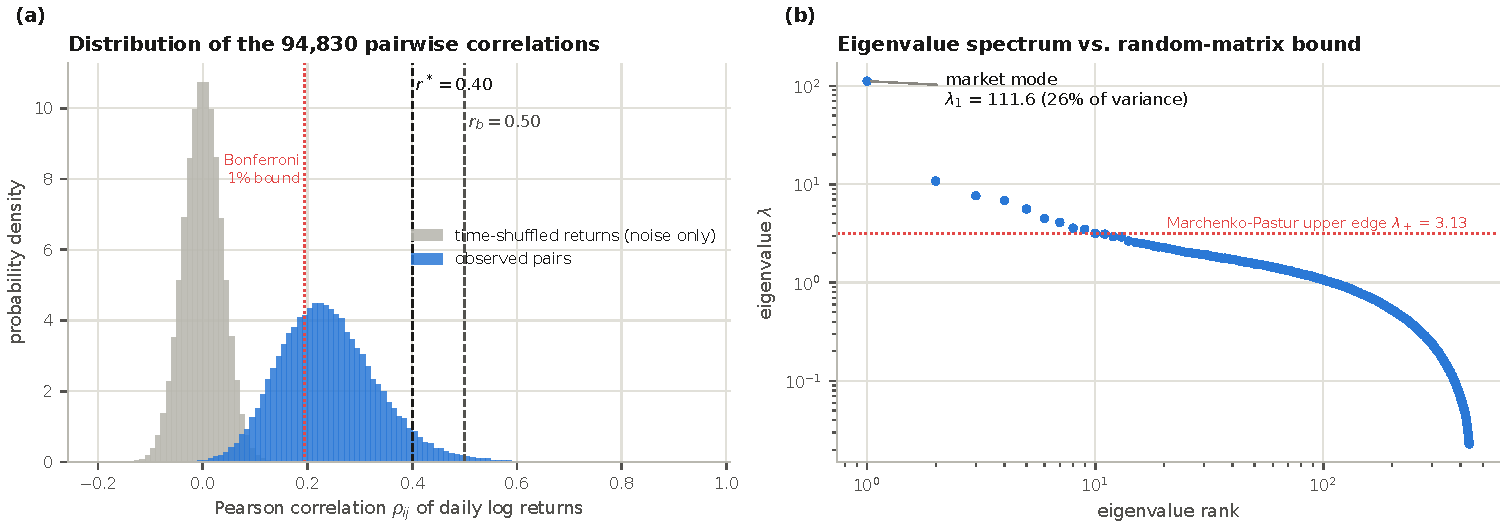
\includegraphics[width=\textwidth]{fig01_correlation_overview.pdf}
\caption{(a) Pairwise correlations of daily log returns against the time-shuffled null. Dashed lines mark the two
working thresholds, the dotted line the Bonferroni-corrected 1\% significance bound. (b) Eigenvalues of the correlation
matrix on log--log axes; the dotted line is the largest eigenvalue compatible with uncorrelated returns.}
\label{fig:corr}
\end{figure}

The sector-ordered correlation matrix (Figure~\ref{fig:heat}) anticipates the homophily results. Diagonal blocks are
visible for IT, FMCG, healthcare, metals and cement, but the dominant visual feature is the bands of uniformly high
correlation that cut across sectors (financials, metals, oil and gas, power, construction), while IT, FMCG and
healthcare are pale against everything except themselves.

\begin{figure}[H]
\centering
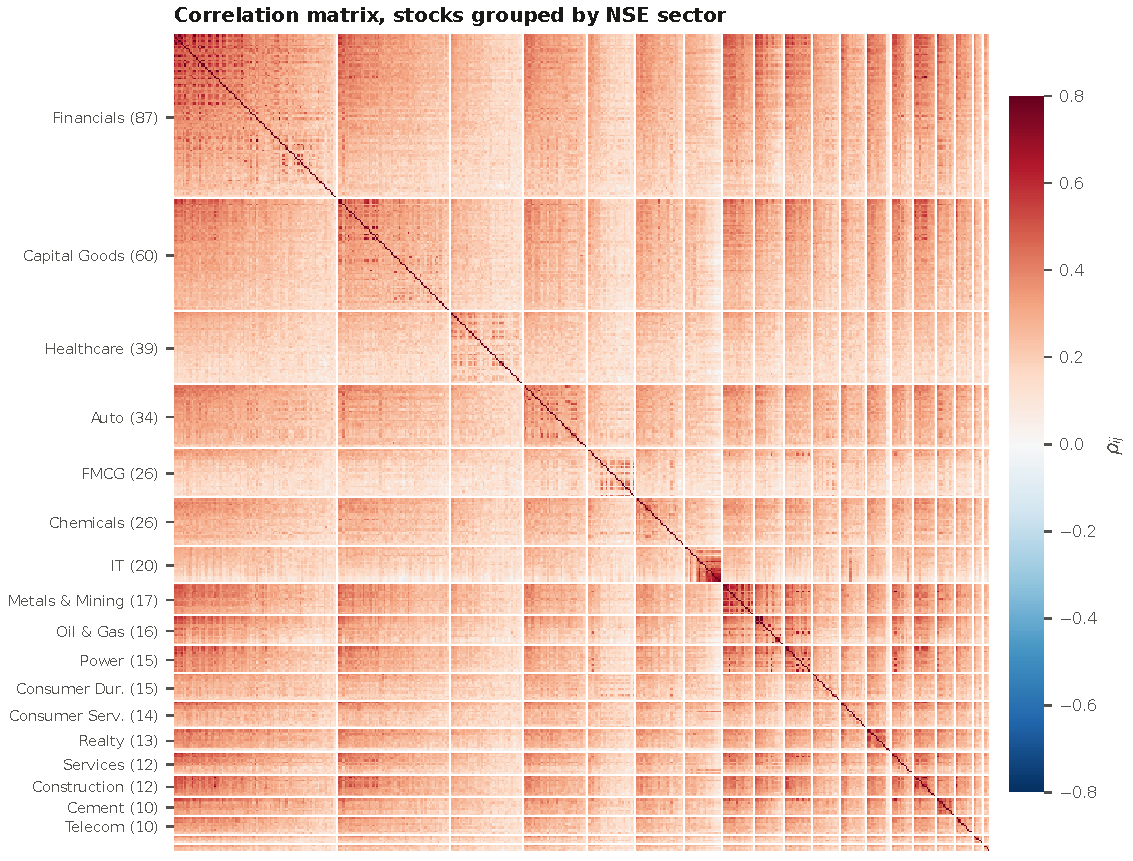
\includegraphics[width=0.74\textwidth]{fig02_correlation_heatmap.pdf}
\caption{Correlation matrix with stocks grouped by NSE sector (sectors ordered by size; within a sector, stocks are
ordered by their mean correlation with the market). Labels are shown for sectors with at least nine stocks.}
\label{fig:heat}
\end{figure}

% ---------------------------------------------------------------------------
\subsection{A. Degree distribution}\label{sec:degree}

\textbf{Linear scale.} At $\rstar$ the mean degree is \valf{A.star_mean}{1} but the median is only \valf{A.star_median}{0}:
\vali{A.star_isolated} stocks (\valratio{A.star_isolated}{A.star_n}{0}) have no edge at all, while the best-connected
stock has \vali{A.star_max} neighbours (Figure~\ref{fig:degree}(a)). A random graph with the same number of nodes and
edges would have a binomial degree distribution with standard deviation \valf{A.star_er_sd}{1}, essentially no isolated
node, and an expected maximum degree of about \vali{A.star_er_max_expected}. The observed standard deviation is
\valf{A.star_sd}{1}. The top 10\% of stocks hold \valp{A.star_top10pct_share}{0} of all edge end-points and the Gini
coefficient of degree is \valf{A.star_gini}{2}. In the backbone the inequality is sharper still
(\vali{A.back_isolated} isolated stocks, maximum degree \vali{A.back_max}, Gini \valf{A.back_gini}{2}). The
distribution is therefore very far from the random-graph (Poisson-like) case: the first alternative in the assignment's
question is ruled out.

\begin{figure}[H]
\centering
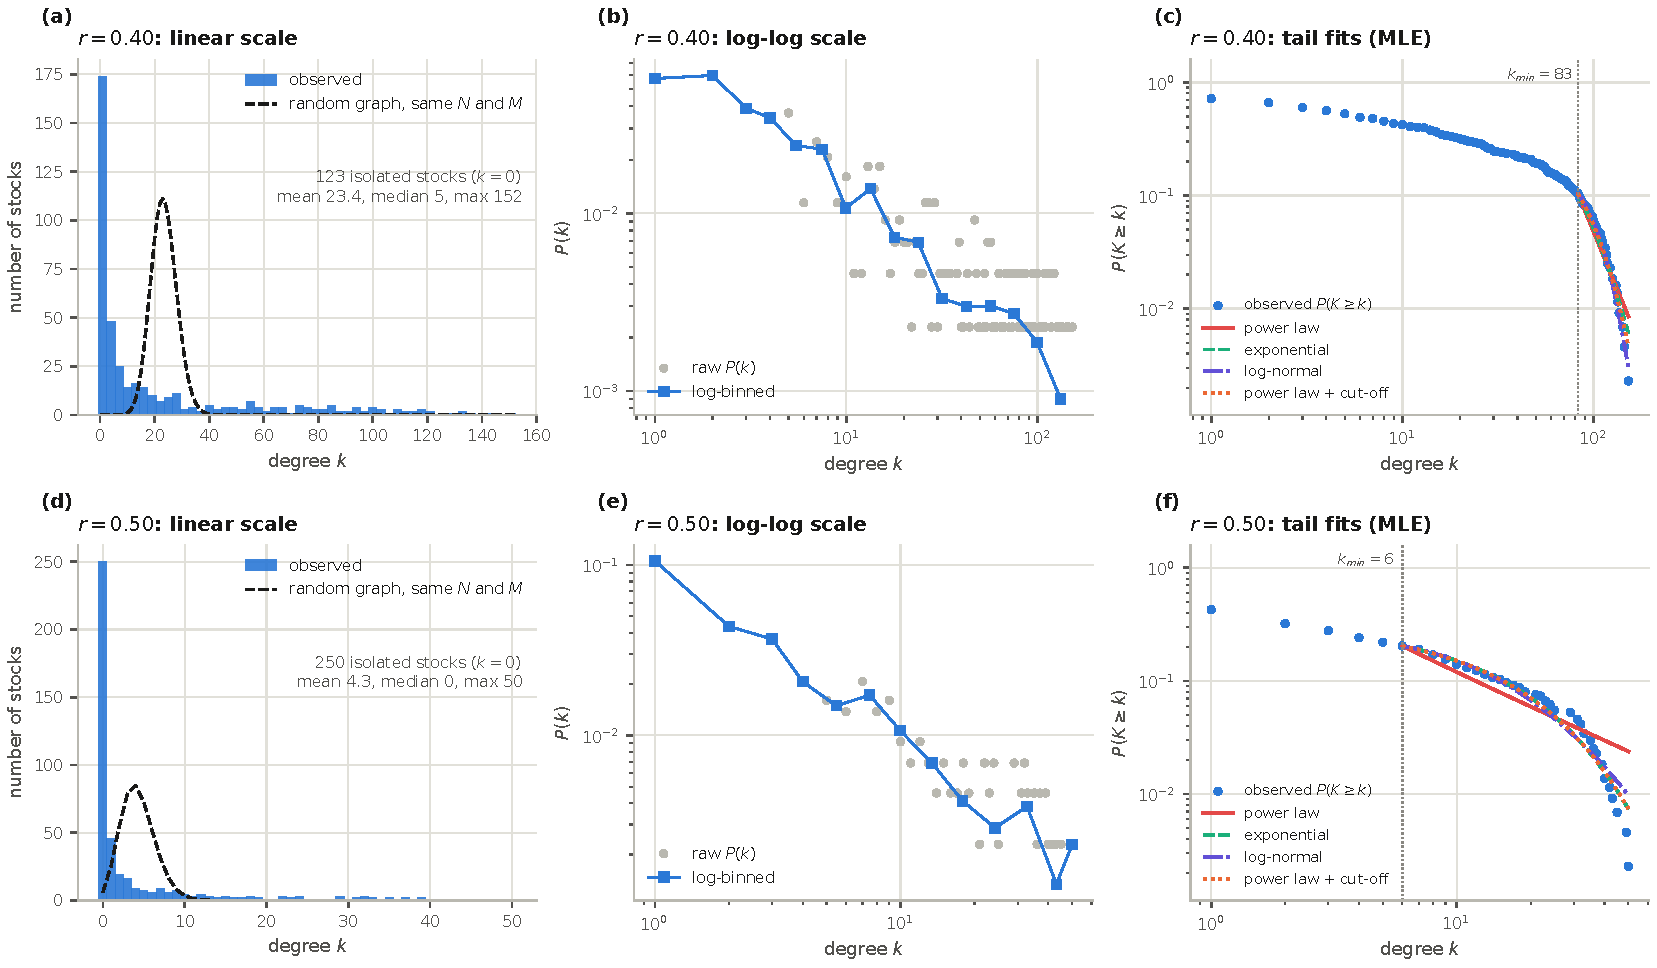
\includegraphics[width=\textwidth]{fig03_degree_distribution.pdf}
\caption{Degree distribution at $\rstar=0.40$ (top) and $\rback=0.50$ (bottom). Left: linear scale with the binomial
distribution of a random graph of equal density. Centre: $P(k)$ on log--log axes, raw and logarithmically binned.
Right: complementary cumulative distribution with maximum-likelihood fits to the tail $k\ge k_{\min}$.}
\label{fig:degree}
\end{figure}

\textbf{Log--log scale.} Does that make it scale-free? Panels (b) and (e) of Figure~\ref{fig:degree} show a decreasing
trend that could be mistaken for a power law over about one decade, but the cumulative plots in panels (c) and (f) bend
downwards, which a power law does not do. The formal test confirms the visual impression (Table~\ref{tab:tailfits}).

\begin{itemize}
\item At $\rstar$ the best power-law fit starts at $k_{\min}=\vali{A.star_kmin}$, covers only \vali{A.star_ntail} stocks
and has the implausible exponent $\alpha=\valf{A.star_alpha}{1}$; its goodness-of-fit $p$-value is \valf{A.star_gof_p}{3},
below the 0.1 rejection level. The exponential is preferred by Vuong's test ($p\approx\valf{A.star_p_exp}{3}$).
\item In the backbone a longer tail is available ($k_{\min}=\vali{A.back_kmin}$, \vali{A.back_ntail} stocks,
$\alpha=\valf{A.back_alpha}{2}$), but the power law is rejected even more clearly ($p<0.01$) and the exponential beats it
by a log-likelihood ratio of \valf{A.back_llr_exp}{1}.
\item Fitted to all connected stocks ($k\ge1$), the power law with exponential cut-off,
$P(k)\propto k^{-\alpha}e^{-\lambda k}$, has the lowest AIC at both thresholds. At $\rstar$ it gives
$\alpha=\valf{A.star_full_tpl_alpha}{2}$ and a cut-off scale $1/\lambda\approx\valf{A.star_full_cutoff_scale}{0}$:
a slow, sub-scale-free decay up to a characteristic degree, and a fast decay beyond it.
\end{itemize}

\begin{table}[H]
\centering\small
\caption{Candidate models for the degree distribution. Columns 3--6 refer to the tail $k\ge k_{\min}$ selected for the
power law: log-likelihood, AIC difference from the best model, log-likelihood ratio of the power law against the model
(negative values favour the alternative) and Vuong's two-sided $p$-value. The last column is the AIC difference when all
models are fitted to the full range $k\ge1$.}\label{tab:tailfits}
\begin{adjustbox}{max width=\linewidth}
\begin{tabular}{clrrrrr}
\toprule
$r$ & Model & $\ln L$ & $\Delta$AIC (tail) & LLR & $p$ & $\Delta$AIC ($k\ge1$)\\
\midrule
\tabinput{tab_tailfits}
\bottomrule
\end{tabular}
\end{adjustbox}
\end{table}

\textbf{Dependence on the threshold.} Tse et al.~\cite{tse2010} observed that scale-free behaviour emerges at high
thresholds, so the test was repeated on a ladder of thresholds (Table~\ref{tab:ladder}). The power law is formally
not rejected at only \vali{A.ladder_n_pl_plausible} of \vali{A.ladder_n} thresholds, and in neither case is the
result informative: at $r=0.30$ the ``tail'' is the top 43 stocks with a fitted exponent at the upper bound of the
search, and at $r=0.60$ it consists of 35 stocks spanning degrees 5 to 13; in both, the exponential fits at least as
well. There is no threshold at which the Nifty~500 network is convincingly scale-free.

\begin{table}[H]
\centering\footnotesize
\caption{Power-law test across thresholds. $N_{k>0}$: connected stocks; $n_{\text{tail}}$: stocks with $k\ge k_{\min}$;
$p_{\text{gof}}$: bootstrap goodness-of-fit from 300 samples ($<0.1$ rejects the power law); LLR and $p$: power law against exponential.}
\label{tab:ladder}
\begin{adjustbox}{max width=\linewidth}
\begin{tabular}{crrrrrrrrrl}
\toprule
$r$ & $N_{k>0}$ & $\avg{k}$ & $k_{\max}$ & $k_{\min}$ & $n_{\text{tail}}$ & $\alpha$ & $p_{\text{gof}}$ & LLR & $p$ & Best (AIC)\\
\midrule
\tabinput{tab_ladder}
\bottomrule
\end{tabular}
\end{adjustbox}
\end{table}

\textbf{Answer to A.} The degree distribution is strongly right-skewed and far broader than a random graph's, with a
small set of stocks holding a large share of the links, but its tail is exponentially bounded. It is a ``broad-scale''
network, not a scale-free one. Section~\ref{sec:market} explains why: degree is almost a deterministic function of a
single bounded quantity, the stock's correlation with the market.

% ---------------------------------------------------------------------------
\subsection{B. Centrality leaderboard}\label{sec:centrality}

Table~\ref{tab:leader} lists the ten highest-ranked stocks on each centrality in the primary network; the backbone
leaderboard is in the Appendix (Table~\ref{tab:leaderback}).

\begin{table}[H]
\centering\footnotesize
\caption{Top-10 stocks by degree, betweenness and eigenvector centrality at $\rstar=0.40$. An asterisk marks
public-sector undertakings (PSUs).}\label{tab:leader}
\setlength{\tabcolsep}{4pt}
\begin{adjustbox}{max width=\linewidth}
\begin{tabular}{r lll lll lll}
\toprule
 & \multicolumn{3}{c}{Degree centrality} & \multicolumn{3}{c}{Betweenness centrality} & \multicolumn{3}{c}{Eigenvector centrality}\\
\cmidrule(lr){2-4}\cmidrule(lr){5-7}\cmidrule(lr){8-10}
\# & Stock & Sector & Value & Stock & Sector & Value & Stock & Sector & Value\\
\midrule
\tabinput{tab_leaderboard_star}
\bottomrule
\end{tabular}
\end{adjustbox}
\end{table}

\textbf{Degree: who moves with the most peers?} The leader is DLF (real estate), linked to
\valp{B.star_top1_deg_value}{0} of all other stocks, followed by IRCTC, Container Corporation, Canara Bank, NCC, Tata
Power and REC. Two things are notable. First, the ten names come from \vali{B.star_top_sectors_deg} different
sectors: a hub is not the centre of its own industry but a stock that moves with everything. Second,
\vali{B.star_psu_in_top_deg} of the ten are government-owned, although PSUs are only \valratio{data.n_psu}{data.n_stocks}{0}
of the nodes (hypergeometric $p=\valf{B.star_psu_top_deg_p}{4}$); in the backbone the count is
\vali{B.back_psu_in_top_deg} of ten. The mean degree of a PSU is \valf{B.star_psu_mean_degree}{0} against
\valf{B.star_private_mean_degree}{0} for a private-sector stock.

\textbf{Eigenvector: who is connected to the well-connected?} The eigenvector list shares
\vali{B.star_overlap_deg_eig} of its ten names with the degree list and the two rankings are almost identical across all
stocks (Spearman $\rho_s=\valf{B.star_sp_deg_eig}{2}$). This near-redundancy is itself a structural statement: there is
one dense core, and having many neighbours means being in it. The $k$-core decomposition says the same thing: the
innermost core has \vali{B.star_n_max_core} stocks each linked to at least \vali{B.star_max_core} of the others.

\textbf{Betweenness: who bridges?} Here the picture changes completely. Only \vali{B.star_overlap_deg_btw} of the ten
betweenness leaders are degree leaders, and \vali{B.star_n_btw_zero} stocks have betweenness exactly zero. The top three,
Indian Hotels, Eternal (formerly Zomato) and Info Edge, form a chain, and the reason they rank first is specific and
checkable (Figure~\ref{fig:central}(a)). At $\rstar$ the IT sector forms a tight cluster with
\vali{B.it_external_edges} edges to non-IT stocks in total. One of the few paths out runs from the IT cluster to Info
Edge (whose recruitment business depends on IT hiring), from Info Edge to Eternal (in which Info Edge is a large
shareholder), and from Eternal to Indian Hotels, which is embedded in the core. Eternal has degree
\vali{B.bridge_ETERNAL_degree}, and yet removing it would detach \vali{B.bridge_ETERNAL_cut} stocks,
\vali{B.bridge_ETERNAL_cut_sector_n} of them IT, from the giant component. Betweenness thus identifies not the
important stocks but the \emph{thin places} of the network; the corridor between the export-oriented IT sector and the
domestic economy is one stock wide. Laurus Labs and Aarti Industries rank highly for the same reason: many of the shortest paths into the pharmaceutical
and chemical stocks pass through them.

\begin{figure}[H]
\centering
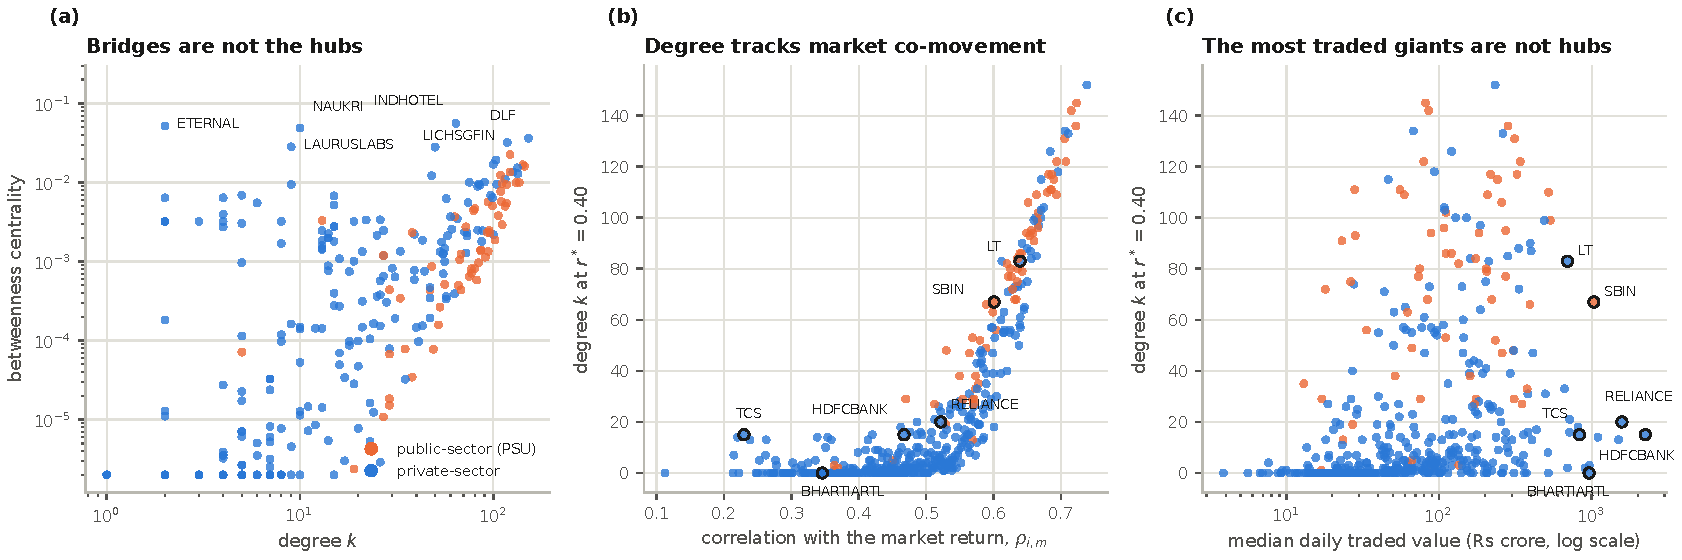
\includegraphics[width=\textwidth]{fig04_centrality.pdf}
\caption{Centrality at $\rstar=0.40$. (a) Betweenness against degree for connected stocks (log axes; zero betweenness is
drawn at the bottom). (b) Degree against the stock's correlation with the equal-weighted market return. (c) Degree against
median daily traded value. Six index heavyweights are circled.}
\label{fig:central}
\end{figure}

\textbf{Do the leaders match the index heavyweights?} They do not (Table~\ref{tab:heavy}). The twelve heavyweights
have a median degree rank of \valf{B.heavy_median_rank_deg}{0} out of \vali{data.n_stocks}; only
\vali{B.heavy_in_top50} of them (\val{B.heavy_best_rank_name}, rank \vali{B.heavy_best_rank_deg}) is in the top fifty, and
\vali{B.heavy_isolated} (Bharti Airtel and ITC) have no edge at all. Reliance has \vali{B.RELIANCE_degree} neighbours,
HDFC Bank \vali{B.HDFCBANK_degree} and TCS \vali{B.TCS_degree}. TCS and Infosys also show why eigenvector centrality must
be read with care: they are well connected inside IT, but IT sits outside the core, so their eigenvector score is
essentially zero.

\begin{table}[H]
\centering\footnotesize
\caption{Index heavyweights in the network at $\rstar=0.40$. ``Size rank'' is the rank by median daily traded value
among the \vali{data.n_stocks} stocks; $\rho_{im}$ is the correlation with the equal-weighted market return. Ranks are out of
\vali{data.n_stocks}; the last column is the degree in the backbone.}\label{tab:heavy}
\begin{adjustbox}{max width=\linewidth}
\begin{tabular}{llrrrrrrr}
\toprule
Stock & Sector & Size rank & $\rho_{im}$ & $k$ & Degree rank & Betw.\ rank & Eigenv.\ rank & $k$ at $\rback$\\
\midrule
\tabinput{tab_heavy}
\bottomrule
\end{tabular}
\end{adjustbox}
\end{table}

The explanation is in Figure~\ref{fig:central}(b). Degree is a steep, almost deterministic function of
$\rho_{im}$, the stock's correlation with the equal-weighted market return (Spearman
$\rho_s=\valf{B.star_sp_deg_rhom}{2}$): the \vali{B.star_n_rhom_lt050} stocks with $\rho_{im}<0.5$ have a median degree of
\valf{B.star_median_degree_rhom_lt050}{0}, and every stock with $\rho_{im}>0.68$ has at least
\vali{B.star_min_degree_rhom_gt068} neighbours. The ten degree leaders have an average $\rho_{im}$ of \valf{B.top10_mean_rho_market}{2}; the
heavyweights average \valf{B.heavy_mean_rho_market}{2}, below the all-stock mean of
\valf{B.all_mean_rho_market}{2}. Size and liquidity do help in general: the rank correlation between degree and traded value is
\valf{B.star_sp_deg_size}{2}, falling to \valf{B.star_sp_deg_size_connected}{2} among connected stocks, since the
isolated stocks are mostly small and illiquid. But the very largest names are scattered along the bottom of Figure~\ref{fig:central}(c). In a network where
every stock has one vote, centrality measures how closely a stock tracks the \emph{typical} stock, not how much capital
it represents. Section~\ref{sec:disc-central} returns to this.

% ---------------------------------------------------------------------------
\subsection{C. Clustering and sector homophily}\label{sec:clustering}

\textbf{How clustered is the network?} At $\rstar$ the average local clustering coefficient is
$\avg{C}=\valf{C.star_avg_clustering}{3}$ over all \vali{data.n_stocks} stocks and \valf{C.star_avg_clustering_deg2}{3} over
the \vali{C.star_n_deg2plus} stocks with at least two neighbours; the transitivity is \valf{C.star_transitivity}{3}. The
network contains \vali{C.star_triangles} triangles. Table~\ref{tab:clust} places these numbers against the two
random-graph references.

\begin{table}[H]
\centering\small
\caption{Clustering and path length against random references (mean of 200 graphs each). ER: same $N$ and $M$.
Rewired: same degree sequence. Path lengths are within the giant component.}\label{tab:clust}
\begin{adjustbox}{max width=\linewidth}
\begin{tabular}{lrrrrrr}
\toprule
 & \multicolumn{3}{c}{$\rstar=0.40$} & \multicolumn{3}{c}{$\rback=0.50$}\\
\cmidrule(lr){2-4}\cmidrule(lr){5-7}
 & Observed & ER & Rewired & Observed & ER & Rewired\\
\midrule
Average clustering $\avg{C}$ & \valf{C.star_avg_clustering}{3} & \valf{C.star_er_clustering}{3} & \valf{C.star_cm_clustering}{3}
 & \valf{C.back_avg_clustering}{3} & \valf{C.back_er_clustering}{3} & \valf{C.back_cm_clustering}{3}\\
Transitivity & \valf{C.star_transitivity}{3} & \valf{C.star_er_transitivity}{3} & \valf{C.star_cm_transitivity}{3}
 & \valf{C.back_transitivity}{3} & \valf{C.back_er_transitivity}{3} & \valf{C.back_cm_transitivity}{3}\\
Average path length & \valf{C.star_apl}{2} & \valf{C.star_er_apl}{2} & \valf{C.star_cm_apl}{2}
 & \valf{C.back_apl}{2} & \valf{C.back_er_apl}{2} & \valf{C.back_cm_apl}{2}\\
Giant-component fraction & \valp{C.star_gcc_frac}{0} & \valp{C.star_er_gcc_frac}{0} & -- & \valp{C.back_gcc_frac}{0} & \valp{C.back_er_gcc_frac}{0} & --\\
\bottomrule
\end{tabular}
\end{adjustbox}
\end{table}

The transitivity is about ten times that of a random graph of equal density, with a path length only
\valf{C.star_l_ratio}{2} times longer: by the usual criterion~\cite{watts1998,humphries2008} this is a small-world
network (small-world index $\sigma=\valf{C.star_sigma}{1}$). But the degree-preserving reference shows that this
comparison flatters the network. Simply giving the nodes their observed degrees and wiring them at random already
yields a transitivity of \valf{C.star_cm_transitivity}{2}, because the hubs are so numerous that they are bound to be
linked to one another. Roughly four-fifths of the observed clustering is a consequence of the degree sequence; the
genuine excess is the step from \valf{C.star_cm_transitivity}{2} to \valf{C.star_transitivity}{2}
($z=\valf{C.star_cm_transitivity_z}{0}$ against the rewired ensemble). In the backbone the excess is larger,
\valf{C.back_cm_transitivity}{2} to \valf{C.back_transitivity}{2}.

\textbf{Individual nodes.} Local clustering \emph{decreases} with degree (Figure~\ref{fig:clust}(a), Spearman
$\rho_s=\valf{C.star_ck_spearman}{2}$). Stocks with fewer than ten neighbours average $C_i=\valf{C.star_low_mean_c}{2}$
and \vali{C.star_n_c_one} of them have $C_i=1$: their few neighbours are all mutually linked, typically sector peers.
The \vali{C.star_n_hubs50} stocks with $k\ge50$ average \valf{C.star_hub_mean_c}{2}, and the largest hub,
\val{C.star_lowest_c_hub}, has the lowest value among them, \valf{C.star_lowest_c_hub_value}{2}: its
\vali{C.star_lowest_c_hub_degree} neighbours come from many groups that are not all linked to each other. A falling
$C(k)$ is the signature of a hierarchical organisation, with tight groups at the periphery connected through a looser
core.

\begin{figure}[H]
\centering
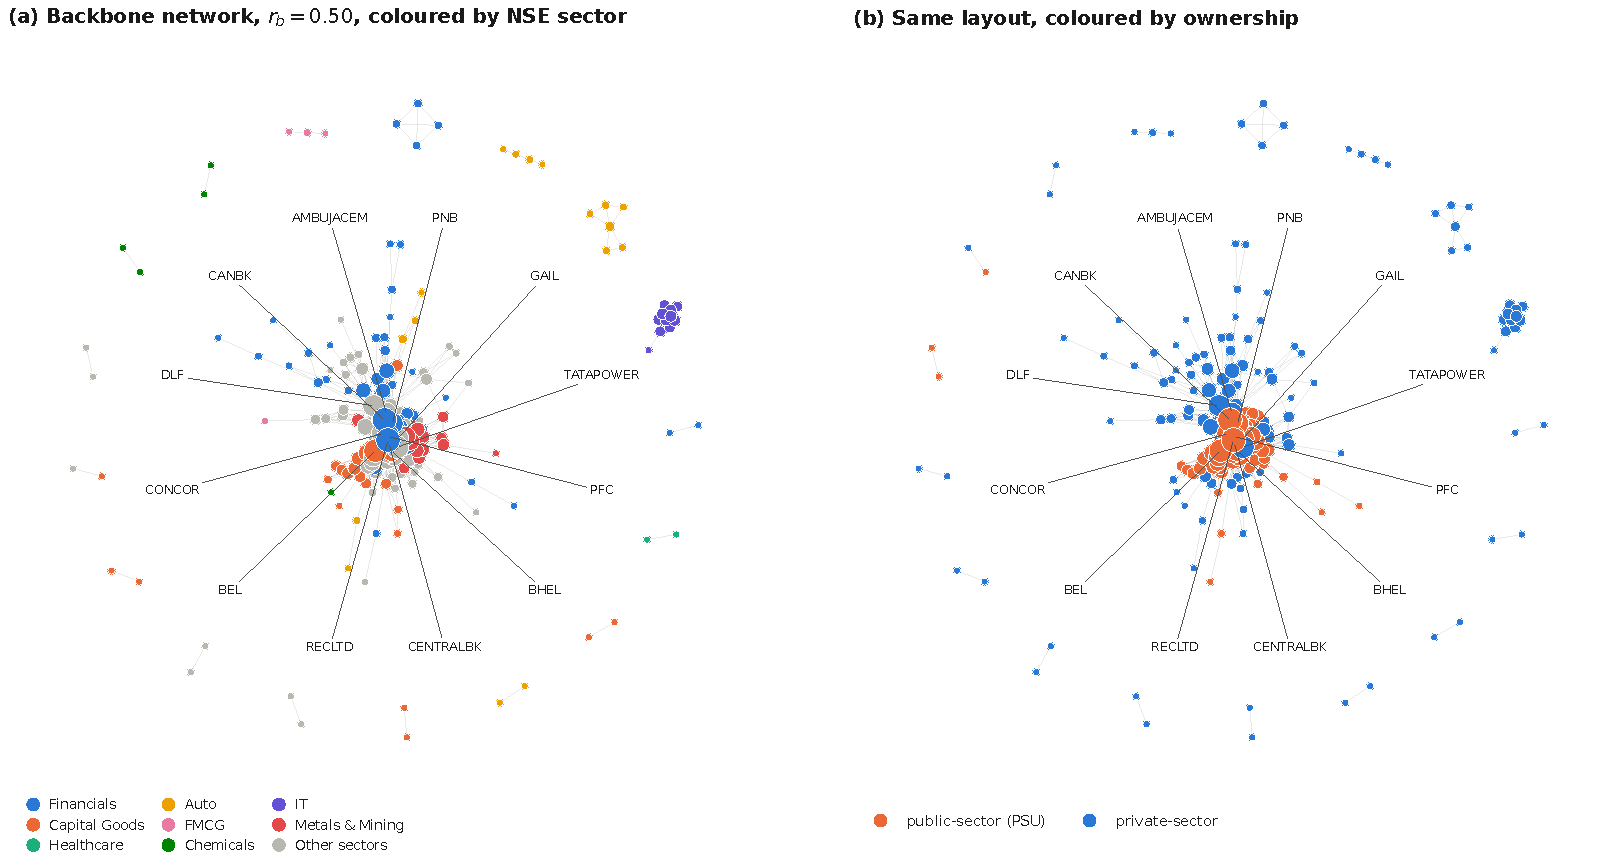
\includegraphics[width=\textwidth]{fig05_network_backbone.pdf}
\caption{The backbone network ($\rback=0.50$; \vali{A.back_n_connected} connected stocks, \vali{D.r50_edges} edges;
isolated stocks not drawn). Node area is proportional to degree; the twelve highest-degree stocks are labelled. The same
layout is coloured (a) by NSE sector, the eight largest sectors in colour, and (b) by ownership.}
\label{fig:net}
\end{figure}

\textbf{Do triangles form inside sectors?} Yes, significantly, but less than one might expect. At $\rstar$,
\valp{C.star_sector_intra_fraction}{1} of edges join two stocks of the same NSE sector, against
\valp{C.star_sector_expected_uniform}{1} if edges ignored sectors ($z=\valf{C.star_edge_z}{0}$ under label shuffling,
$p<0.001$). Of the \vali{C.star_tri_total} triangles, \valp{C.star_tri_mono_frac}{1} lie entirely within one sector
against \valp{C.star_tri_mono_null}{1} under the null ($z=\valf{C.star_tri_mono_z}{0}$), a six-fold enrichment
(Figure~\ref{fig:clust}(d)). The majority of triangles, \valratio{C.star_tri_mixed}{C.star_tri_total}{0}, nevertheless
connect three \emph{different} sectors, and the sector assortativity coefficient is a modest
\valf{C.star_sector_assortativity}{3}. Homophily strengthens as the threshold rises: in the backbone
\valp{C.back_sector_intra_fraction}{0} of edges and \valp{C.back_tri_mono_frac}{0} of triangles are within-sector and the
assortativity is \valf{C.back_sector_assortativity}{2}.

\begin{figure}[H]
\centering
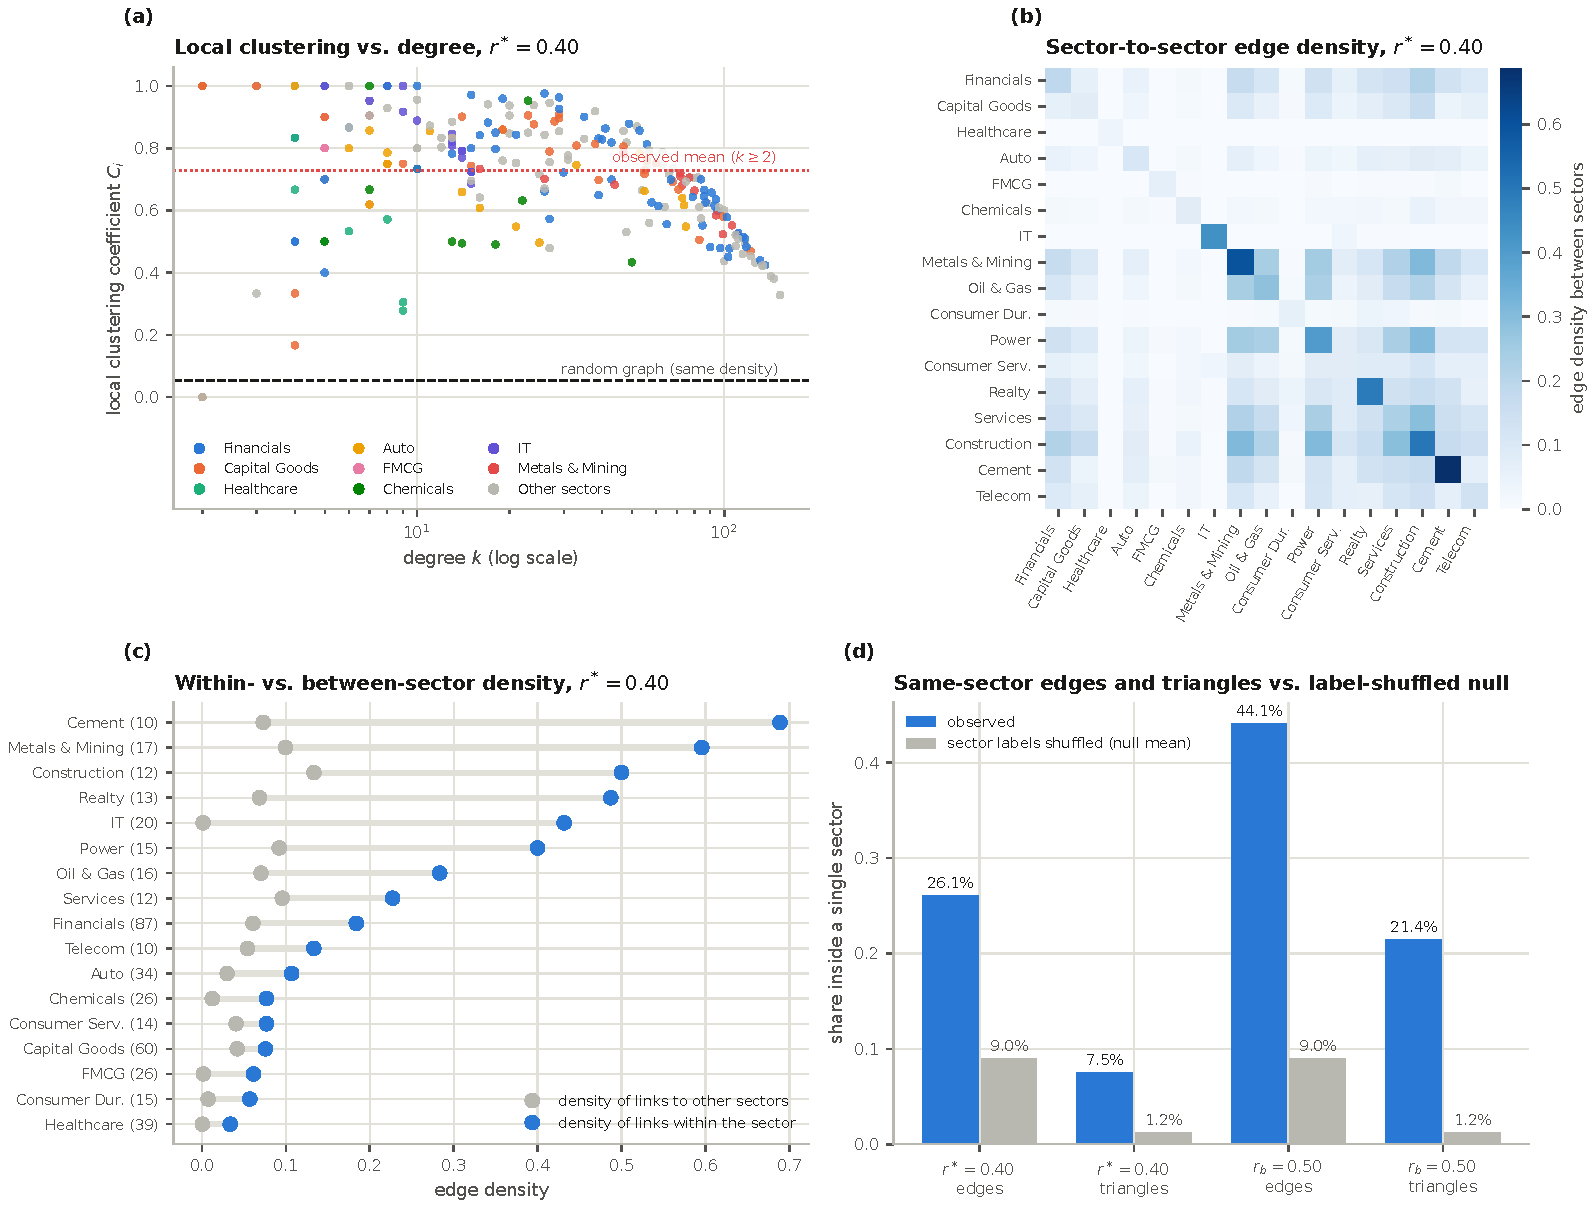
\includegraphics[width=\textwidth]{fig06_clustering_homophily.pdf}
\caption{Clustering and sector homophily. (a) Local clustering coefficient against degree at $\rstar$. (b) Edge density
between each pair of sectors. (c) Edge density within each sector compared with its density of links to other sectors
(sector size in brackets). (d) Share of edges and triangles lying inside a single sector, observed against the mean of
2{,}000 label shuffles.}
\label{fig:clust}
\end{figure}

\textbf{Sectors differ sharply} (Table~\ref{tab:sectors}, Figure~\ref{fig:clust}(b,c)), and fall into three types.

\begin{itemize}
\item \emph{Self-contained sectors.} IT is the clearest case: \valp{C.star_it_internal_density}{0} of IT pairs are linked
but only \valp{C.star_it_external_density}{1} of IT--non-IT pairs, a ratio of more than 300. In the backbone IT is a
separate eleven-stock component with no link to the rest (the violet cluster in Figure~\ref{fig:net}(a)). FMCG behaves
similarly on a smaller scale: at $\rstar$ eight consumer-staples companies
(\val{C.star_second_comp_members}) form the only component other than the giant one.
\item \emph{Dense but outward-looking sectors.} Cement, metals and mining, construction, realty and power have internal
densities of 0.4--0.7 \emph{and} many external links. Their off-diagonal blocks in Figure~\ref{fig:clust}(b) are as dark
as some sectors' diagonals. These are the domestic cyclicals that make up the core.
\item \emph{Sectors that barely exist as network objects.} Healthcare has \vali{C.star_health_n} stocks, of which
\vali{C.star_health_isolated} are isolated at $\rstar$, and an internal density of
\valf{C.star_health_internal_density}{3}; consumer durables and FMCG are similar. Their stocks are not uncorrelated with
their peers, but their correlations rarely reach 0.4.
\end{itemize}

\begin{table}[H]
\centering\footnotesize
\caption{Sector cohesion at $\rstar=0.40$ for sectors with at least nine stocks. ``Ratio'' is internal over external
density; $\avg{C}_{k\ge2}$ is the mean local clustering of the sector's stocks with at least two neighbours. The last
column is the internal density in the backbone.}\label{tab:sectors}
\begin{adjustbox}{max width=\linewidth}
\begin{tabular}{lrrrrrrrrr}
\toprule
 & & & Mean & Internal & \multicolumn{2}{c}{Edge density} & & & Internal\\
\cmidrule(lr){6-7}
Sector & Stocks & Isolated & degree & edges & internal & external & Ratio & $\avg{C}_{k\ge2}$ & density at $\rback$\\
\midrule
\tabinput{tab_sector_cohesion}
\bottomrule
\end{tabular}
\end{adjustbox}
\end{table}

\textbf{A second label: ownership.} Figure~\ref{fig:net}(b) recolours the backbone by whether the company is a
public-sector undertaking (a hand-compiled flag for the \vali{data.n_psu} government-controlled companies in the
sample), and the core turns almost uniformly orange. The numbers are striking:

\begin{itemize}
\item \valp{C.star_psu_internal_density}{0} of all PSU--PSU pairs are linked at $\rstar$, and
\valp{C.back_psu_internal_density}{0} even at $\rback$, where the overall density is \valp{C.back_density}{1}.
\item PSU--PSU pairs are \fpeval{round(100*(\rawval{data.n_psu}*(\rawval{data.n_psu}-1)/2)/\rawval{data.n_pairs},1)}\% of all
pairs but \valp{C.back_psu_edges_share}{0} of backbone edges, and \valp{C.back_tri_psu_only_frac}{0} of backbone triangles
consist of three PSUs.
\item Not one PSU is isolated at $\rstar$; in the backbone \vali{C.back_psu_in_gcc} of the \vali{data.n_psu} are in the
giant component and make up \valp{C.back_psu_share_of_gcc}{0} of it.
\item The ownership assortativity is \valf{C.back_psu_assortativity}{2} in the backbone, higher than the sector
assortativity of \valf{C.back_sector_assortativity}{2}, although ownership is a two-valued label and sector a
twenty-valued one.
\item The backbone contains \vali{C.back_n_max_cliques} heavily overlapping cliques of \vali{C.back_max_clique} stocks, in
each of which every pair is correlated above 0.5. One of them is \val{C.back_max_clique_members}:
\vali{C.back_max_clique_psu} of its members are PSUs, and they span \vali{C.back_max_clique_sectors} NSE sectors
(financials, which here means banks and power and housing financiers, together with oil and gas, power, cement,
construction and logistics).
\end{itemize}

\textbf{Answer to C.} The network is highly clustered, but most of that clustering follows from its hub-dominated degree
sequence. Triangles are enriched within sectors by a factor of six, and for IT, cement, metals and realty the sector is
a real network community. The single most cohesive group of stocks, however, is defined by state ownership and cuts
across sectors.

% ---------------------------------------------------------------------------
\subsection{D. Threshold sensitivity}\label{sec:sweep}

The network was rebuilt for \vali{D.grid_n} thresholds between \valf{D.grid_min}{2} and \valf{D.grid_max}{2}.
Table~\ref{tab:sweep} gives the values at round thresholds and Figure~\ref{fig:sweep} the full curves.

\begin{table}[H]
\centering\footnotesize
\caption{The network at seven thresholds. APL and diameter are measured within the giant component (GC).
$\avg{C}$ averages over all \vali{data.n_stocks} stocks; the last column is the same-sector share of edges.}\label{tab:sweep}
\begin{adjustbox}{max width=\linewidth}
\begin{tabular}{crrrrrrrrrrr}
\toprule
$r$ & Edges & Density (\%) & $\avg{k}$ & Isolated & GC & GC (\%) & APL & Diam. & $\avg{C}$ & Transit. & Same sector (\%)\\
\midrule
\tabinput{tab_sweep}
\bottomrule
\end{tabular}
\end{adjustbox}
\end{table}

\begin{figure}[H]
\centering
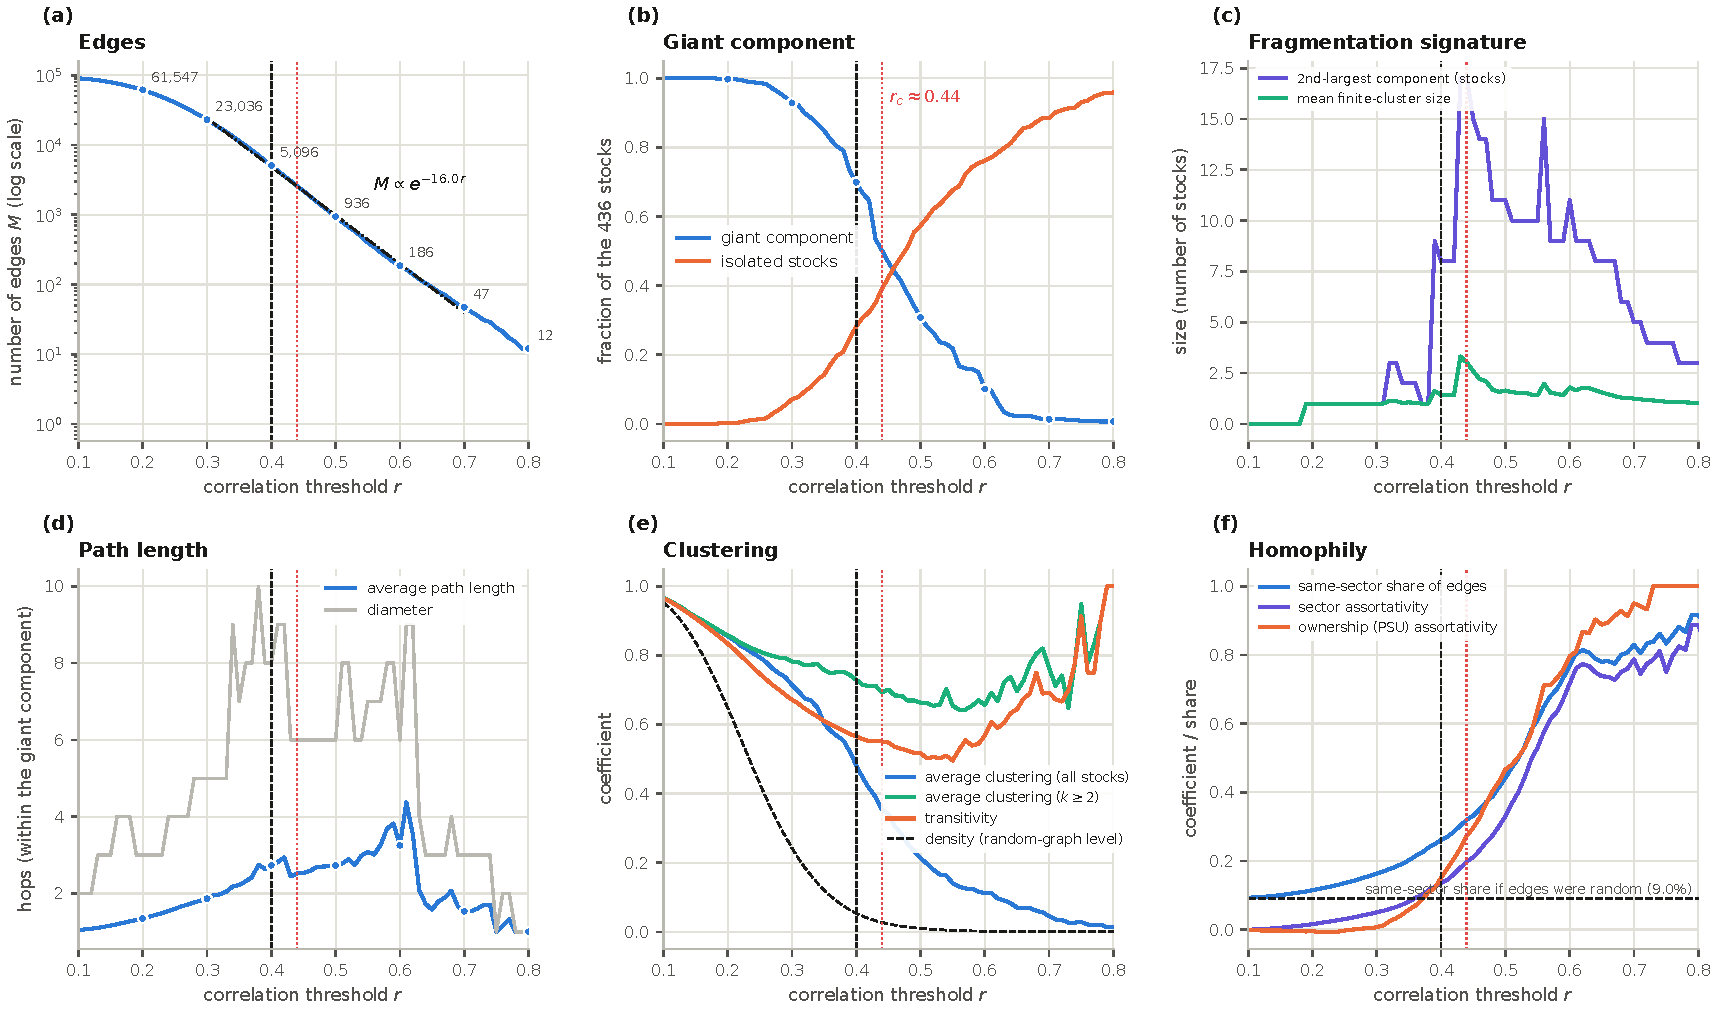
\includegraphics[width=\textwidth]{fig07_threshold_sensitivity.pdf}
\caption{Threshold sweep. The dashed vertical line is $\rstar=0.40$ and the dotted line the point
$r_c\approx\valf{D.r_half}{2}$ at which the giant component falls below half of the stocks. Markers show the round
thresholds of Table~\ref{tab:sweep}.}
\label{fig:sweep}
\end{figure}

\textbf{Edges.} Between $r=0.3$ and $r=0.7$ the number of edges falls exponentially, $M\propto e^{-\valf{D.edge_decay_rate}{1}\,r}$
(Figure~\ref{fig:sweep}(a)): each increase of $0.1$ in $r$ divides the edge count by \valf{D.edge_factor_per_0p1}{1}, and it
halves every \valf{D.edge_halving_dr}{3}. Moving the primary threshold by only $\pm0.02$ changes the network from
\vali{D.star_edges_minus} to \vali{D.star_edges_plus} edges. The definition of a ``connection'' is therefore anything but
innocuous: a reader who prefers $r=0.38$ to $r=0.42$ gets twice as many links.

\textbf{Giant component.} Connectivity does not collapse at a sharp point (Figure~\ref{fig:sweep}(b)). The network is
fully connected only up to $r=\valf{D.r_fully_connected_max}{2}$; the giant component still holds 90\% of stocks at
$r=\valf{D.r_gcc90}{2}$, half at $r_c=\valf{D.r_half}{2}$, 10\% at $r=0.60$, and is gone by $0.70$. Its decline is mirrored
by the rise in isolated stocks, and the second-largest component never exceeds \vali{D.second_peak_size} stocks
(Figure~\ref{fig:sweep}(c)). The network does not break into large pieces; it is \emph{eroded}, losing peripheral stocks
one by one while a core stays connected.

Figure~\ref{fig:gcc} makes the same point against a random graph. At $r_c$ the mean degree is still
\valf{D.mean_degree_at_rc}{1}. An Erd\H{o}s--R\'enyi graph with that mean degree would have essentially every node in its
giant component (it only fragments near $\avg{k}=1$), whereas here half the stocks are already disconnected. The edges
are so concentrated in the core that a high average degree coexists with a large disconnected periphery.

\begin{figure}[H]
\centering
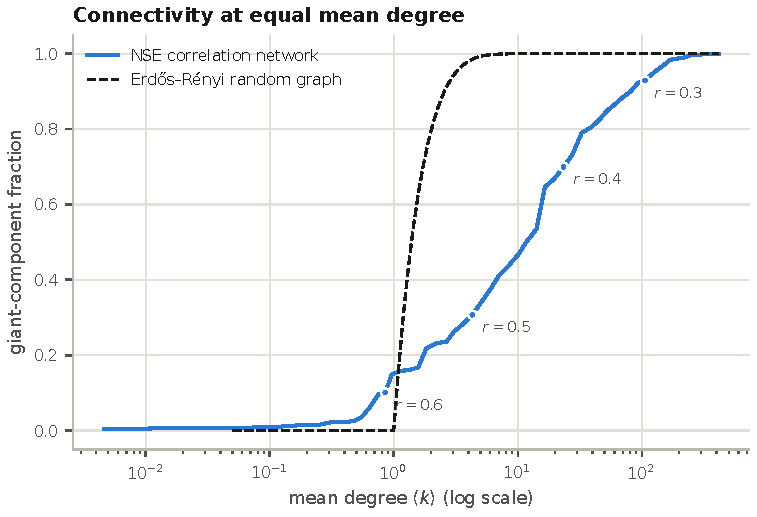
\includegraphics[width=0.56\textwidth]{fig08_giant_component_vs_random.pdf}
\caption{Giant-component fraction as a function of mean degree: the observed network along the threshold sweep against the
Erd\H{o}s--R\'enyi result $S=1-e^{-\avg{k}S}$.}
\label{fig:gcc}
\end{figure}

\textbf{Average path length.} The path length is not monotonic in $r$ (Figure~\ref{fig:sweep}(d)). It rises from
\valf{D.r20_apl}{2} at $r=0.2$ to \valf{D.r40_apl}{2} at $r=0.4$ as shortcuts are removed, stays between about 2.4 and 2.9 from 0.4 to
0.5 while the periphery is being shed (the surviving core is compact), peaks at \valf{D.apl_peak}{2} at
$r=\valf{D.apl_peak_r}{2}$, where the giant component is a stringy remnant of about forty stocks, and then falls only
because the component itself shrinks to a handful of nodes. A short path length at high $r$ is thus not a sign of
efficiency; it is measured on a different and much smaller object. The diameter reaches its maximum of
\vali{D.diameter_max} at $r=\valf{D.diameter_max_r}{2}$, while long chains of peripheral stocks are still attached to the core.

\textbf{Clustering and homophily.} Transitivity stays between \valf{D.transitivity_min}{2} and 0.85 over the whole range
$0.2\le r\le0.7$ while the density falls by three orders of magnitude (Figure~\ref{fig:sweep}(e)): triangles are a
property of the correlation structure, not of density. The average clustering over all stocks falls steadily, but only
because isolated stocks contribute zeros. Sector homophily rises monotonically, from \valp{D.r20_intra}{0} of edges at
$r=0.2$ to \valp{D.r60_intra}{0} at $r=0.6$ (Figure~\ref{fig:sweep}(f)). The threshold acts as a lens: at low $r$ the
network shows the market, at high $r$ it shows industries and, above 0.7, individual pairs of twin companies.

\textbf{Answer to D.} Connectivity is fragile to the definition of an edge in terms of size (five-fold fewer edges per
0.1) but robust in terms of organisation: at every threshold between 0.3 and 0.6 there is a single dense core with an
unconnected periphery, high transitivity and positive homophily. What changes is how much of the market is admitted
to the core.

% ---------------------------------------------------------------------------
\subsection{Extension E1: how much of the network is ``the market''?}\label{sec:market}

\textbf{A single factor predicts the hubs.} The correlation of each stock with the equal-weighted market return ranges
from \valf{E1.rho_m_min}{2} to \valf{E1.rho_m_max}{2} (mean \valf{E1.rho_m_mean}{2}), and is higher for PSUs
(\valf{E1.rho_m_psu_mean}{2}) than for private-sector stocks (\valf{E1.rho_m_private_mean}{2}). Thresholding the one-factor
matrix of Eq.~\eqref{eq:onefactor} at $\rstar$ produces a network of \vali{E1.star_of_edges_one} edges that can be laid
over the observed \vali{E1.star_of_edges_obs}:

\begin{itemize}
\item \valp{E1.star_of_precision}{0} of the edges the market factor predicts are present in the data, and they account for
\valp{E1.star_of_recall}{0} of the observed edges.
\item The predicted and observed degree sequences have a rank correlation of \valf{E1.star_of_degree_spearman}{2}
(Figure~\ref{fig:market}(a)). \emph{Who} the hubs are is essentially decided by one number per stock.
\item The one-factor network is itself highly clustered (transitivity \valf{E1.star_of_one_transitivity}{2}) and has no
sector homophily (assortativity \valf{E1.star_of_one_sector_assort}{2}). High clustering therefore requires no sector
structure at all: under Eq.~\eqref{eq:onefactor} an edge exists when $\rho_{im}\rho_{jm}>r$, so the neighbourhoods are
nested and the stocks with the highest $\rho_{im}$ form a clique.
\end{itemize}

This also explains result~A. Under the one-factor model the degree of stock $i$ is the number of stocks $j$ with
$\rho_{jm}>r/\rho_{im}$: a deterministic, steeply increasing function of a quantity that is bounded above by one and
has a bell-shaped distribution across stocks. Such a mechanism generates a broad degree distribution with a hard
upper cut-off, which is what Section~\ref{sec:degree} found; it cannot generate the unbounded tail of a scale-free
network.

\textbf{What the market factor does not explain.} Almost all observed degrees lie \emph{above} the diagonal in
Figure~\ref{fig:market}(a): \vali{E1.star_of_excess_edges} edges exist beyond the one-factor prediction, and
\valp{E1.star_of_excess_same_sector}{0} of them are within-sector, twice the share among the edges the factor does explain
(\valp{E1.star_of_explained_same_sector}{0}). In the backbone the market factor predicts just \vali{E1.back_of_edges_one}
edges (\valp{E1.back_of_recall}{1} of those observed). Of the \vali{E1.back_of_excess_edges} others,
\valp{E1.back_of_excess_same_sector}{0} are within-sector and \valp{E1.back_of_excess_psu_pair}{0} join two PSUs. The
backbone is thus almost entirely the structure \emph{beyond} the market: the second layer of factors.

\begin{figure}[H]
\centering
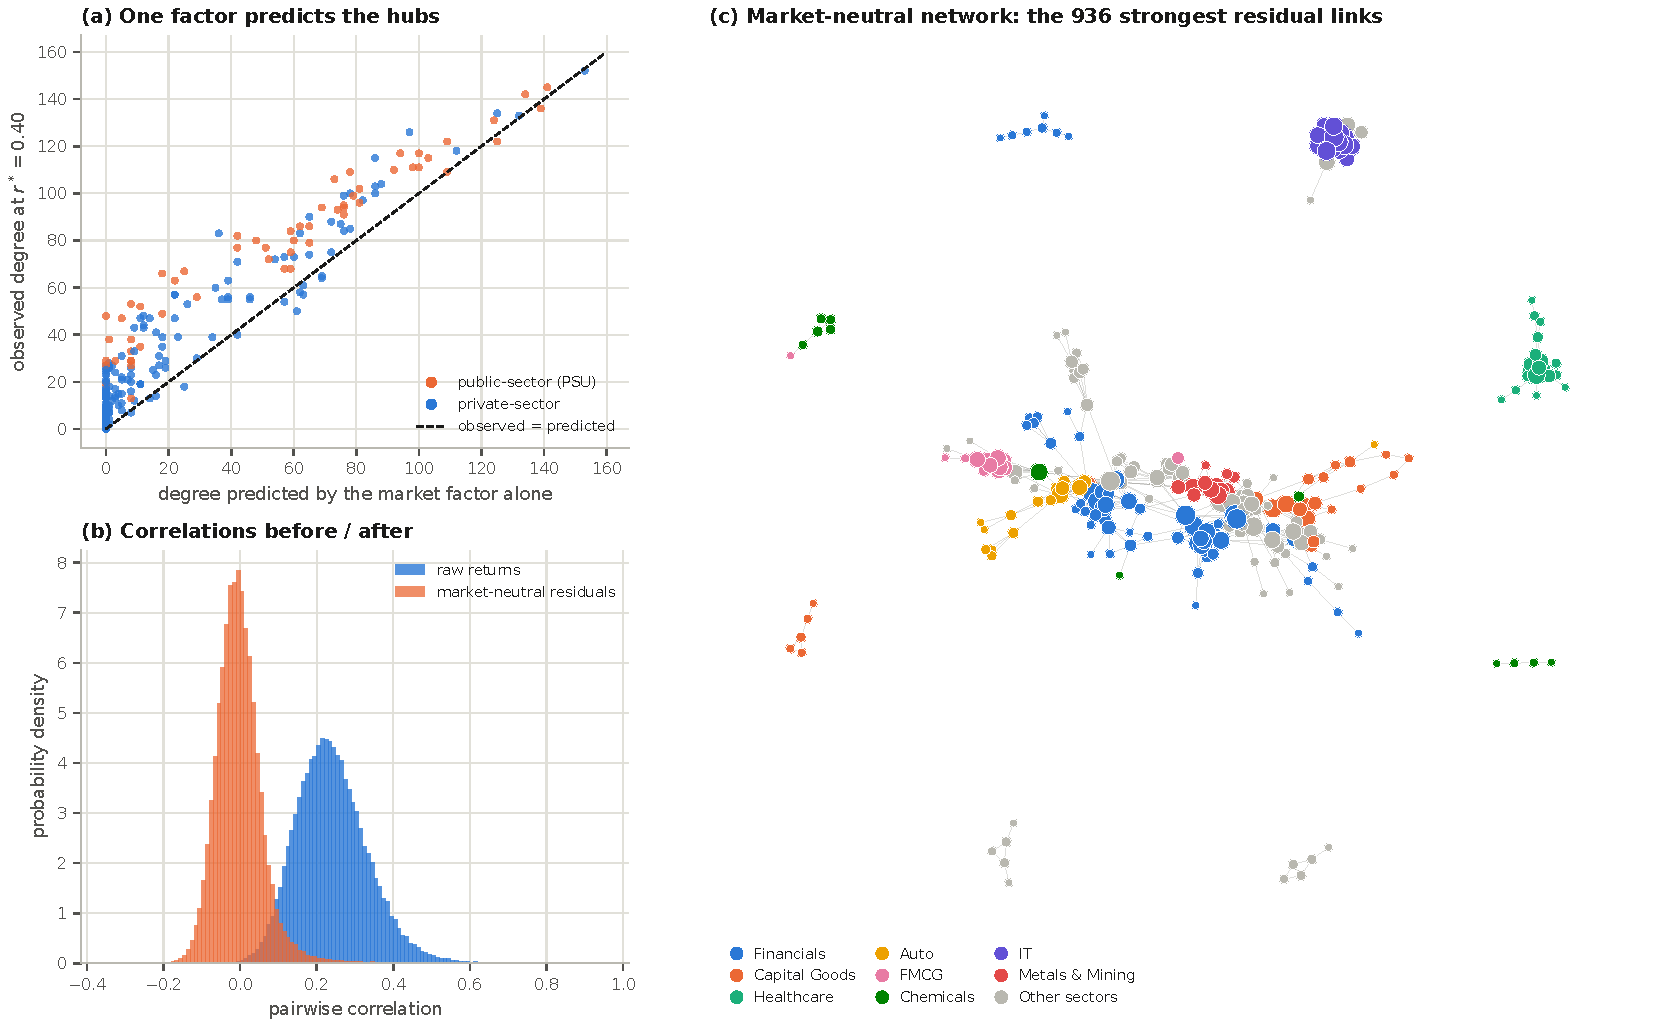
\includegraphics[width=\textwidth]{fig09_market_mode.pdf}
\caption{The market mode. (a) Observed degree at $\rstar$ against the degree predicted by the single-index model.
(b) Pairwise correlations of raw returns and of market-neutral residuals. (c) Network of the residuals, thresholded to
keep the same number of edges as the backbone; components of at least three stocks, coloured by sector.}
\label{fig:market}
\end{figure}

\textbf{The market-neutral network.} After regressing the market return out of every stock, the residual correlations are
centred on zero (mean \valf{E1.res_mean}{3}, standard deviation \valf{E1.res_sd}{3}; Figure~\ref{fig:market}(b)).
Table~\ref{tab:residual} compares raw and residual networks at equal numbers of edges.

\begin{table}[H]
\centering\small
\caption{Raw and market-neutral networks at matched density.}\label{tab:residual}
\begin{adjustbox}{max width=\linewidth}
\begin{tabular}{lrrrr}
\toprule
 & \multicolumn{2}{c}{Matched to $\rstar$} & \multicolumn{2}{c}{Matched to $\rback$}\\
\cmidrule(lr){2-3}\cmidrule(lr){4-5}
 & Raw & Residual & Raw & Residual\\
\midrule
\tabinput{tab_residual}
\bottomrule
\end{tabular}
\end{adjustbox}
\end{table}

Three changes are worth stating. \emph{The hubs disappear}: with the same \vali{E1.star_raw_edges} edges, no stock is
isolated any more, the maximum degree halves from \vali{E1.star_raw_max_degree} to \vali{E1.star_res_max_degree} and the
Gini coefficient of degree falls from \valf{E1.star_raw_degree_gini}{2} to \valf{E1.star_res_degree_gini}{2}.
\emph{Sectors appear}: sector assortativity more than doubles at both densities, and at backbone density
\valp{E1.back_res_mono_sector_triangles}{0} of triangles lie within one sector (\valp{E1.back_raw_mono_sector_triangles}{0}
before). Healthcare, nearly invisible in the raw network, becomes a cohesive group; in
Figure~\ref{fig:market}(c) pharmaceuticals, IT, FMCG, autos and metals are each a distinct cluster. \emph{The PSU group
survives}: ownership assortativity \emph{rises} to \valf{E1.star_res_psu_assortativity}{2} and
\valf{E1.back_res_psu_assortativity}{2}. The PSU effect is therefore not just a matter of PSUs being high-beta stocks;
they share a common component of return that is separate from the market.

% ---------------------------------------------------------------------------
\subsection{Extension E2: how reliable is the network?}\label{sec:stability}

\textbf{Sampling uncertainty.} Across 500 block-bootstrap resamples of the trading days the number of edges at $\rstar$
has a 95\% interval of \vali{E2.star_boot_edges_lo} to \vali{E2.star_boot_edges_hi} (coefficient of variation
\valp{E2.star_boot_edges_cv}{0}) around the full-sample value of \vali{D.r40_edges}; in the backbone it runs from
\vali{E2.back_boot_edges_lo} to \vali{E2.back_boot_edges_hi} (Figure~\ref{fig:stability}(a)). The giant component holds between
\valp{E2.star_boot_gcc_lo}{0} and \valp{E2.star_boot_gcc_hi}{0} of the stocks. The edges that \emph{are} in the full-sample
network are individually fairly reliable: on average each appears in \valp{E2.star_edge_retention_mean}{0} of the
replicates, and only \valp{E2.star_edge_retention_lt50}{1} appear in fewer than half
(Figure~\ref{fig:stability}(b)). The uncertainty is in how many \emph{additional} pairs cross the threshold, which
depends on how often the resample happens to draw the few most turbulent days.

\textbf{The leaderboard.} The identity of the hubs is more stable than the size of the network. DLF is among the ten
highest-degree stocks in \valp{E2.star_top1_freq}{0} of replicates, and \vali{E2.star_n_ever_gt50} stocks are in the top
ten more often than not (Table~\ref{tab:boot} in the Appendix). But ranks 8--10 of Table~\ref{tab:leader} are not
distinguishable from ranks 11--20: the least stable member of the full-sample top ten appears there in only
\valp{E2.star_top10_min_freq}{0} of replicates, and the bootstrap standard deviation of a hub's degree is about 40.
The leaderboard should be read as a group of roughly fifteen interchangeable names, not as a strict ranking.

\begin{figure}[H]
\centering
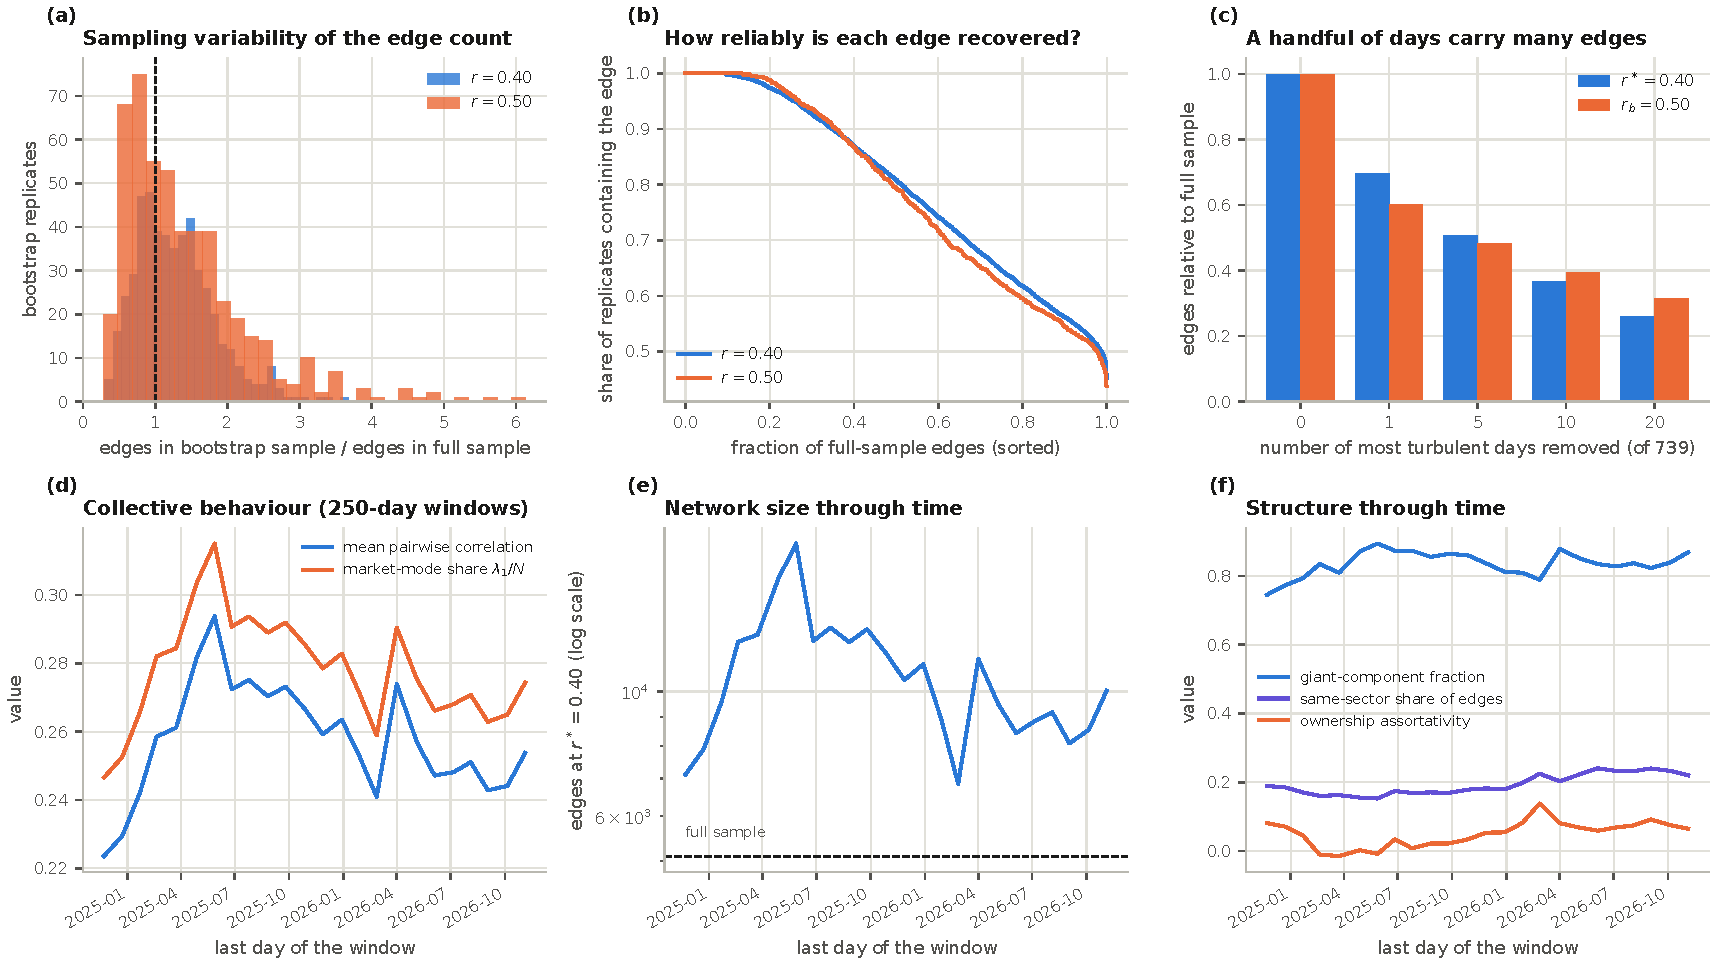
\includegraphics[width=\textwidth]{fig10_stability.pdf}
\caption{Reliability of the network. (a) Bootstrap distribution of the edge count relative to the full sample.
(b) For each full-sample edge, the share of bootstrap replicates in which it reappears. (c) Edges remaining after removing the
days with the largest absolute market return. (d)--(f) Rolling 250-day windows, plotted at the last day of each window.}
\label{fig:stability}
\end{figure}

\textbf{A few days carry the network.} The largest market move in the sample is 4~June 2024, the day the
general-election results were declared: the equal-weighted market fell \fpeval{round(abs(\rawval{E2.worst_day_return_pct}),1)}\%,
the average PSU \fpeval{round(abs(\rawval{E2.worst_day_psu_return_pct}),1)}\% and the average private-sector stock
\fpeval{round(abs(\rawval{E2.worst_day_private_return_pct}),1)}\%. Deleting that single observation, 0.14\% of the
sample, removes \valf{E2.drop1_edge_loss_pct_star}{0}\% of the edges at $\rstar$ and
\valf{E2.drop1_edge_loss_pct_back}{0}\% of the backbone (Table~\ref{tab:turbulent}, Figure~\ref{fig:stability}(c)). Deleting
the twenty most turbulent days (2.7\% of the sample) removes \valf{E2.drop20_edge_loss_pct_star}{0}\% and
\valf{E2.drop20_edge_loss_pct_back}{0}\%. This is the known tendency of correlations to be driven by high-volatility
periods~\cite{forbes2002}, seen here at the level of individual edges.

\begin{table}[H]
\centering\footnotesize
\caption{Effect of deleting the $n$ days with the largest absolute equal-weighted market return. ``Top-10'' is the
number of full-sample top-10 degree stocks still in the top ten.}\label{tab:turbulent}
\begin{adjustbox}{max width=\linewidth}
\begin{tabular}{rr rrrrr rrrrr}
\toprule
 & & \multicolumn{5}{c}{$\rstar=0.40$} & \multicolumn{5}{c}{$\rback=0.50$}\\
\cmidrule(lr){3-7}\cmidrule(lr){8-12}
Days & Mean & & & \multicolumn{2}{c}{Assortativity} & & & & \multicolumn{2}{c}{Assortativity} & \\
\cmidrule(lr){5-6}\cmidrule(lr){10-11}
removed & $\rho$ & Edges & GC & sector & PSU & Top-10 & Edges & GC & sector & PSU & Top-10\\
\midrule
\tabinput{tab_turbulent}
\bottomrule
\end{tabular}
\end{adjustbox}
\end{table}

Two details in Table~\ref{tab:turbulent} sharpen the interpretation. First, sector and ownership assortativity
\emph{increase} as turbulent days are removed (at $\rstar$, from \valf{C.star_psu_assortativity}{2} to
\valf{E2.drop20_psu_assort_star}{2} for ownership). Crash days add links indiscriminately, because everything falls
together; they are responsible for the cross-sector edges of the core, not for the sector and PSU groups, which
are a calm-market feature. Second, the degree leaderboard at $\rstar$ is fairly robust (\vali{E2.drop1_top10_overlap_star}
of ten names survive the removal of 4~June 2024), whereas the backbone leaderboard is not
(\vali{E2.drop1_top10_overlap_back} of ten).

\textbf{Persistence.} Splitting the sample at \val{E2.star_split_split_date} gives \vali{E2.star_split_edges_first} edges in
the first half and \vali{E2.star_split_edges_second} in the second at $\rstar$, with a Jaccard overlap of only
\valf{E2.star_split_edge_jaccard}{2}; the two halves' correlation matrices have a correlation of
\valf{E2.star_split_corr_of_correlations}{2} and their degree sequences a rank correlation of
\valf{E2.star_split_degree_spearman}{2}. Who is central persists moderately well; which exact pairs are linked does not.

\textbf{Time variation.} In rolling 250-day windows the mean correlation moves between \valf{E2.roll_meancorr_min}{2} and
\valf{E2.roll_meancorr_max}{2} and the edge count at $\rstar$ between \vali{E2.roll_edges_min} and \vali{E2.roll_edges_max}, a
factor of \valf{E2.roll_edges_ratio}{1} (Figure~\ref{fig:stability}(d,e)). The largest single change is the fall from
\vali{E2.roll_edges_last_with_worst} to \vali{E2.roll_edges_first_without_worst} edges between the windows ending
\val{E2.roll_last_with_worst} and \val{E2.roll_first_without_worst}, which is when 4~June 2024 leaves the window. A second
observation is methodological: \emph{every} one-year window has more edges than the three-year network. A shorter
window gives noisier correlation estimates, with a wider distribution and therefore more of them above any fixed
threshold, and it does not average over regimes. A threshold is consequently not portable across window lengths, and
networks built with ``$r=0.5$'' from one and from three years of data are not comparable.

% ===========================================================================
\section{Interpretation and Discussion}\label{sec:discussion}
% ===========================================================================

\subsection{What kind of network is this?}

The picture that emerges from A, C and D together is a \textbf{core--periphery} network, not a scale-free one and not
a modular one. A core of roughly a hundred stocks is densely interlinked across sector boundaries; around it lie a few
tight sector clusters attached by thin bridges (IT, autos, private-sector life insurers, FMCG); and beyond those,
a periphery of between a quarter and more than half of the market, depending on the threshold, that is linked to no one. The evidence is the degree
distribution with its mass at zero and its bounded tail, the near-identity of degree and eigenvector centrality, the
erosion (not fragmentation) of the giant component as $r$ rises, the falling $C(k)$, and the very high mean degree
at which the network disconnects.

The reason is the correlation structure of Section~\ref{sec:corr}. When one factor carries a quarter of the variance
and the next carries a tenth of that, the strongest correlations are mostly between the stocks most exposed to the
first factor. A threshold then selects a set of mutually connected high-exposure stocks, and that set is the core.
The scale-free picture of Tse et al.~\cite{tse2010}, obtained for the full US market of many thousands of stocks,
does not carry over to a 436-stock emerging-market universe with a dominant market mode, and the formal
test~\cite{clauset2009} rejects it here. This is not unusual: Broido and Clauset~\cite{broido2019} find that
strongly scale-free structure is rare among real networks once it is tested and not assumed.

\subsection{Why the hubs are not the heavyweights}\label{sec:disc-central}

Table~\ref{tab:heavy} would be a puzzle if centrality were read as importance. Reliance, HDFC Bank, ICICI Bank, TCS and
Infosys are the stocks that move the index, yet they sit in the middle or at the edge of the network. Three
considerations resolve it.

\emph{Centrality counts peers, not rupees.} Every stock is one node. A stock has a high degree when it co-moves with
many \emph{other stocks}, and most of the \vali{data.n_stocks} stocks are mid-sized domestic businesses. The equal-weighted
market return, which determines degree almost completely, has a correlation of \valf{E1.ew_vs_nifty500_corr}{2} with the
capitalisation-weighted Nifty~500 index but only \valf{E1.ew_vs_nifty50_corr}{2} with the Nifty~50. The typical stock and
the large-cap index are different things, and the network is a statement about the former.

\emph{The largest companies have their own drivers.} The IT majors earn most of their revenue abroad and respond to
global technology demand and the exchange rate. Reliance is a conglomerate priced on energy margins, telecom and retail.
ITC, Hindustan Unilever and Bharti Airtel are defensive businesses with steady cash flows. Each carries a substantial
component of return that the average domestic stock does not share, which keeps its correlations with most stocks below
0.4. Low centrality here means diversifying, not unimportant.

\emph{The actual hubs are the purest carriers of the domestic cycle.} Real estate (DLF), construction and railways
(NCC, IRCON, Container Corporation, IRCTC), power and its financiers (Tata Power, REC, PFC), public-sector banks
(Canara Bank, PNB) and capital goods (BHEL, BEL) are all leveraged to domestic growth, interest rates and government
capital expenditure. They have little idiosyncratic business risk of the kind that would decouple them from the market.

For a portfolio manager the practical reading is the reverse of the naive one. A high-degree stock is a poor
diversifier, since holding ten of the leaders in Table~\ref{tab:leader} is close to holding one position, and a
leveraged one. The peripheral and isolated stocks are where diversification is available.

\subsection{Sector, ownership and the two layers of structure}

The assignment asks whether triangles form within industries. They do, six times more often than chance, but the more
interesting finding is the ordering of the two labels: state ownership is a stronger predictor of an edge than
industry. A plausible reading is that the market prices PSUs to a considerable extent as a single theme. They share
exposure to government policy on capital expenditure, dividends and disinvestment; many are bought and sold together
through PSU index funds and thematic baskets; and their valuations moved together over the sample period. The
election-result day shows the mechanism at its most extreme, with PSUs falling
\fpeval{round(abs(\rawval{E2.worst_day_psu_return_pct}),0)}\% on average against
\fpeval{round(abs(\rawval{E2.worst_day_private_return_pct}),0)}\% for the rest of the market, but the effect is not an
artefact of that day: PSU assortativity is higher, not lower, when the twenty most turbulent days are removed, and
higher still in the market-neutral network. I cannot separate these explanations with price data alone, and the PSU
flag is my own classification, so this should be read as a well-supported observation with a tentative cause.

More generally, the two extensions show that the network has two layers. The first is the market mode, which decides
who is in the core and produces most of the clustering. The second, visible once the first is removed or when the
threshold is raised, consists of industries and ownership groups. Analyses that stop at the raw threshold network
see mostly the first layer and may attribute to ``sector structure'' what is really common exposure to the market.

\subsection{What the threshold does}

The threshold is not a nuisance parameter to be fixed and forgotten. It selects which layer of the structure is
visible (Figure~\ref{fig:sweep}(f)), and the edge count depends on it exponentially. Two practical consequences
follow. A threshold should be stated as a quantile of the correlation distribution and for a stated window length,
because the same number means different things in different markets and for different sample sizes. And structural
statements should be checked at more than one threshold: here the qualitative conclusions on degree heterogeneity,
the identity of the hubs, clustering and homophily hold at both $0.40$ and $0.50$, while quantitative ones (the number
of edges, the exact ranking, the path length) do not.

\subsection{Limitations}\label{sec:limits}

\begin{itemize}
\item \textbf{Survivorship and look-ahead.} The universe is the Nifty~500 as constituted in November 2026, restricted to
stocks with a full three-year history. Companies that were in the index in 2023 but have since left it are absent, and
\vali{data.n_low_cov} recent listings are excluded. The network describes the established part of today's index.
\item \textbf{Estimation noise.} With $T/N=\valf{data.q_ratio}{2}$ the correlation matrix is noisy; only
\vali{data.n_eig_above_mp} eigenvalues rise above the random-matrix bound. Section~\ref{sec:stability} shows that edge
counts carry sampling errors of 40--60\% and depend heavily on a few days.
\item \textbf{Pearson correlation.} It measures linear, contemporaneous co-movement and is sensitive to extreme
observations. The rank-correlation check and the day-removal experiment bound this problem but do not remove it.
Lead--lag relations and tail dependence are not captured.
\item \textbf{Information discarded.} Thresholding keeps about 5\% of the pairs and treats $\rho=0.41$ and $\rho=0.90$
alike. Weighted or filtered networks would retain more, but were outside the scope set by the assignment.
\item \textbf{Labels.} The sector label is NSE's twenty-way macro classification, which places, for example, Adani
Enterprises in metals and mining and Adani Ports in services although the two have a correlation above 0.8. Business-group
membership, which was not analysed, is clearly a third organising label alongside sector and ownership.
\item \textbf{One regime.} Three years is a single market phase. The rolling analysis shows that the density of the
network varies by a factor of almost three even within it.
\end{itemize}

% ===========================================================================
\section{Conclusion}\label{sec:conclusion}
% ===========================================================================

A correlation-threshold network of \vali{data.n_stocks} Nifty~500 stocks was built from three years of daily returns and
analysed at two thresholds, with null models for every structural claim.

\begin{enumerate}[label=\textbf{\Alph*.}]
\item \textbf{Degree distribution.} It is neither random-like nor scale-free. Degrees range from zero, for
\valratio{A.star_isolated}{A.star_n}{0} of the stocks, to \vali{A.star_max}; a power-law tail is rejected at both
thresholds, and a bounded, cut-off form fits better. The breadth comes from a single market factor acting through a
steep threshold.
\item \textbf{Centrality.} Degree and eigenvector centrality select the same group of domestic-cyclical and
public-sector stocks (DLF, IRCTC, Container Corporation, Canara Bank, REC, Tata Power); betweenness selects the thin
bridges, above all the Info Edge--Eternal--Indian Hotels chain that ties the IT sector to the rest of the market. The
index heavyweights are not central: Reliance, TCS and HDFC Bank rank \vali{B.RELIANCE_rank_deg}, \vali{B.TCS_rank_deg}
and \vali{B.HDFCBANK_rank_deg} of \vali{data.n_stocks} by degree.
\item \textbf{Clustering and homophily.} Transitivity is \valf{C.star_transitivity}{2}, ten times the random-graph value
but only modestly above what the degree sequence implies. Edges and triangles are enriched within sectors by factors
of three and six, and state ownership is an even stronger organising label than sector.
\item \textbf{Threshold sensitivity.} The edge count falls about five-fold per 0.1 increase in $r$; the giant component
erodes gradually and drops below half the market at $r_c\approx\valf{D.r_half}{2}$; the path length is non-monotonic.
The core--periphery organisation itself is stable across thresholds.
\end{enumerate}

The two extensions qualify these answers. The market mode alone reproduces the ranking of the hubs
($\rho_s=\valf{E1.star_of_degree_spearman}{2}$) and most of the clustering, and removing it reveals a second layer of
clean sector clusters. And the network is strongly shaped by a handful of turbulent days, one of which accounts for
\valf{E2.drop1_edge_loss_pct_star}{0}\% of the edges. The main lesson I take from the exercise is that a
threshold network of stock returns is easy to build and easy to over-interpret: its most visible features (hubs, high
clustering, a giant component) can be produced by a single common factor, and it is the comparison with explicit null
models that shows which features carry information about the structure of the economy.

Natural next steps would be to repeat the analysis on intraday (5-minute) returns, where the market mode is weaker; to
add business-group membership as a third label; and to replace the fixed threshold by a statistically validated one that
adapts to the window length.

% ---------------------------------------------------------------------------
\begin{thebibliography}{99}\small
\bibitem{tse2010} C.~K. Tse, J.~Liu and F.~C.~M. Lau, ``A network perspective of the stock market,''
  \emph{Journal of Empirical Finance} \textbf{17}(4), 659--667 (2010).
\bibitem{moghadam2019} H.~E. Moghadam, T.~Mohammadi, M.~F. Kashani and A.~Shakeri, ``Complex networks analysis in Iran
  stock market: The application of centrality,'' \emph{Physica A} \textbf{531}, 121800 (2019).
\bibitem{pan2007} R.~K. Pan and S.~Sinha, ``Collective behavior of stock price movements in an emerging market,''
  \emph{Physical Review E} \textbf{76}, 046116 (2007).
\bibitem{laloux1999} L.~Laloux, P.~Cizeau, J.-P. Bouchaud and M.~Potters, ``Noise dressing of financial correlation
  matrices,'' \emph{Physical Review Letters} \textbf{83}, 1467--1470 (1999).
\bibitem{plerou1999} V.~Plerou, P.~Gopikrishnan, B.~Rosenow, L.~A.~N. Amaral and H.~E. Stanley, ``Universal and
  nonuniversal properties of cross correlations in financial time series,'' \emph{Physical Review Letters}
  \textbf{83}, 1471--1474 (1999).
\bibitem{clauset2009} A.~Clauset, C.~R. Shalizi and M.~E.~J. Newman, ``Power-law distributions in empirical data,''
  \emph{SIAM Review} \textbf{51}(4), 661--703 (2009).
\bibitem{vuong1989} Q.~H. Vuong, ``Likelihood ratio tests for model selection and non-nested hypotheses,''
  \emph{Econometrica} \textbf{57}(2), 307--333 (1989).
\bibitem{broido2019} A.~D. Broido and A.~Clauset, ``Scale-free networks are rare,'' \emph{Nature Communications}
  \textbf{10}, 1017 (2019).
\bibitem{newman2003} M.~E.~J. Newman, ``Mixing patterns in networks,'' \emph{Physical Review E} \textbf{67}, 026126 (2003).
\bibitem{watts1998} D.~J. Watts and S.~H. Strogatz, ``Collective dynamics of `small-world' networks,'' \emph{Nature}
  \textbf{393}, 440--442 (1998).
\bibitem{humphries2008} M.~D. Humphries and K.~Gurney, ``Network `small-world-ness': a quantitative method for
  determining canonical network equivalence,'' \emph{PLoS ONE} \textbf{3}(4), e0002051 (2008).
\bibitem{maslov2002} S.~Maslov and K.~Sneppen, ``Specificity and stability in topology of protein networks,''
  \emph{Science} \textbf{296}, 910--913 (2002).
\bibitem{kunsch1989} H.~R. K\"unsch, ``The jackknife and the bootstrap for general stationary observations,''
  \emph{Annals of Statistics} \textbf{17}(3), 1217--1241 (1989).
\bibitem{sharpe1963} W.~F. Sharpe, ``A simplified model for portfolio analysis,'' \emph{Management Science}
  \textbf{9}(2), 277--293 (1963).
\bibitem{forbes2002} K.~J. Forbes and R.~Rigobon, ``No contagion, only interdependence: measuring stock market
  comovements,'' \emph{Journal of Finance} \textbf{57}(5), 2223--2261 (2002).
\bibitem{networkx} A.~A. Hagberg, D.~A. Schult and P.~J. Swart, ``Exploring network structure, dynamics, and function
  using NetworkX,'' in \emph{Proceedings of the 7th Python in Science Conference (SciPy 2008)}, 11--15 (2008).
\end{thebibliography}

% ===========================================================================
\appendix
\section{Additional tables}\label{app:tables}

\begin{table}[H]
\centering\footnotesize
\caption{Top-10 stocks by centrality in the backbone, $\rback=0.50$. An asterisk marks PSUs.}\label{tab:leaderback}
\setlength{\tabcolsep}{4pt}
\begin{adjustbox}{max width=\linewidth}
\begin{tabular}{r lll lll lll}
\toprule
 & \multicolumn{3}{c}{Degree centrality} & \multicolumn{3}{c}{Betweenness centrality} & \multicolumn{3}{c}{Eigenvector centrality}\\
\cmidrule(lr){2-4}\cmidrule(lr){5-7}\cmidrule(lr){8-10}
\# & Stock & Sector & Value & Stock & Sector & Value & Stock & Sector & Value\\
\midrule
\tabinput{tab_leaderboard_back}
\bottomrule
\end{tabular}
\end{adjustbox}
\end{table}

\begin{table}[H]
\centering\footnotesize
\caption{Stability of the degree leaderboard under the block bootstrap (500 replicates). $k$: full-sample degree;
mean $\pm$ s.d.: bootstrap degree; ``Top-10'': share of replicates in which the stock is among the ten highest
degrees. Stocks are sorted by that share. An asterisk marks PSUs.}\label{tab:boot}
\begin{adjustbox}{max width=\linewidth}
\begin{tabular}{lrrr lrrr}
\toprule
\multicolumn{4}{c}{$\rstar=0.40$} & \multicolumn{4}{c}{$\rback=0.50$}\\
\cmidrule(lr){1-4}\cmidrule(lr){5-8}
Stock & $k$ & Bootstrap $k$ & Top-10 (\%) & Stock & $k$ & Bootstrap $k$ & Top-10 (\%)\\
\midrule
\tabinput{tab_bootstrap}
\bottomrule
\end{tabular}
\end{adjustbox}
\end{table}

\begin{table}[H]
\centering\footnotesize
\begin{minipage}[t]{0.60\textwidth}
\centering
\caption{The twelve most correlated pairs.}\label{tab:pairs}
\begin{adjustbox}{max width=\linewidth}
\begin{tabular}{llr}
\toprule
Pair & Sector(s) & $\rho$\\
\midrule
\tabinput{tab_pairs}
\bottomrule
\end{tabular}
\end{adjustbox}
\end{minipage}\hfill
\begin{minipage}[t]{0.36\textwidth}
\centering
\caption{Sector composition: index, network, and PSUs in the network.}\label{tab:composition}
\begin{adjustbox}{max width=\linewidth}
\begin{tabular}{lrrr}
\toprule
Sector & Index & Network & PSU\\
\midrule
\tabinput{tab_sectors}
\bottomrule
\end{tabular}
\end{adjustbox}
\end{minipage}
\end{table}

\section{Reproducibility}\label{app:repro}

The repository that accompanies this report contains the package \texttt{src/nsenet}, the numbered scripts, the unit
tests, the cached download and, as CSV files, every table behind the figures.

\begin{lstlisting}[language=bash]
pip install -r requirements.txt
python scripts/01_download_data.py   # once; later runs use the cache
python scripts/run_all.py            # steps 02-09, about 6 minutes
python -m pytest -q                  # 20 unit tests on synthetic data
cd report && pdflatex report.tex && pdflatex report.tex
\end{lstlisting}

All random procedures (bootstrap, permutations, random graphs, shuffles) use the fixed seed in \texttt{config.yaml}.
The scripts write every scalar quoted in this report to \texttt{results/numbers/*.json}; step~09 converts those
files into the macros that the \LaTeX{} source reads, so the text cannot drift from the computed values.
Table~\ref{tab:params} lists the settings used.

\begin{table}[H]
\centering\small
\caption{Parameters of the analysis (\texttt{config.yaml}).}\label{tab:params}
\begin{adjustbox}{max width=\linewidth}
\begin{tabular}{ll}
\toprule
Universe / window & Nifty 500; \val{data.first_date} to \val{data.last_date}; daily\\
Minimum price coverage / maximum forward-fill & 97\% of trading days / 3 days\\
Thresholds & $\rstar=\valf{data.r_star}{2}$, $\rback=\valf{data.r_back}{2}$; sweep \valf{D.grid_min}{2}--\valf{D.grid_max}{2}, step \valf{D.grid_step}{2}\\
Random graphs / label permutations / time shuffles & 200 / 2{,}000 / 20\\
Bootstrap & moving blocks of 5 days; 500 replicates\\
Power-law goodness of fit & 500 bootstrap samples (300 per rung of the threshold ladder); tail of at least 25 stocks\\
Rolling windows & \vali{E2.roll_window} trading days, step \vali{E2.roll_step} (\vali{E2.roll_n} windows)\\
Software & Python 3, NetworkX, NumPy, SciPy, pandas, Matplotlib, yfinance \val{data.yfinance_version}\\
\bottomrule
\end{tabular}
\end{adjustbox}
\end{table}

\end{document}
